\chapter[Prospects for $\Htautau$][Prospects for $\Htautau$]{Prospects for $\Htautau$}
\label{chap:prospects}

\begin{quote}
Prospects for the $\Htautau$ analysis in Run-II and at the HL-LHC are described.
\end{quote}

\section{Run-II}
\label{sec:prospects-run2}

In Run-II, the LHC is expected to collide protons with $\sqrt{s} = 13$ TeV, a peak instantaneous luminosity of approximately $1.6\times 10^{34} \text{cm}^{-2} \text{s}^{-1}$, 25 nanosecond bunch spacing, and $\pileup\approx 40$. These data-taking conditions are much harsher than in 2012, as shown in \cref{tab:prospects-datataking}.

\begin{table}[bp] 
  \centering
  \begin{tabular}{c|cccc}
  \hline\hline
  Year of operations      & $\sqrt{s}$ [TeV] & peak lumi. [$\text{cm}^{-2} \text{s}^{-1}$] & bunch spacing [ns] & $\pileup$    \\
  \hline
  2011                    &  7               & $0.4\times 10^{34}$                         & 50                 & $\approx 10$ \\
  2012                    &  8               & $0.8\times 10^{34}$                         & 50                 & $\approx 20$ \\
  2015                    & 13               & $1.6\times 10^{34}$                         & 25                 & $\approx 40$ \\
  \hline\hline
\end{tabular}


  \caption{LHC data-taking conditions in 2011 and 2012 compared with the expected data-taking conditions in 2015.}
  \label{tab:prospects-datataking}
\end{table}

The ATLAS L1 trigger rate would increase by $\approx 5\times$ if the 2012 trigger menu was ported unchanged to 2015 data-taking conditions. However, the L1 bandwidth is expected to increase from 75 kHz to 100 kHz, much less than this rate increase. The L1 menu must then be adapted to accommodate this.

This is especially true of triggers which rely on $\tauh$ since hadronic objects are challenging in the trigger, both in identification and calibration. An unsustainable increase of trigger rate as a function of instantaneous luminosity is shown in \cref{fig:prospects-tautriggerrates}. Multiple avenues were explored to ensure tenable trigger rates without significant loss of physics.

\begin{figure}[tp]
  \centering
  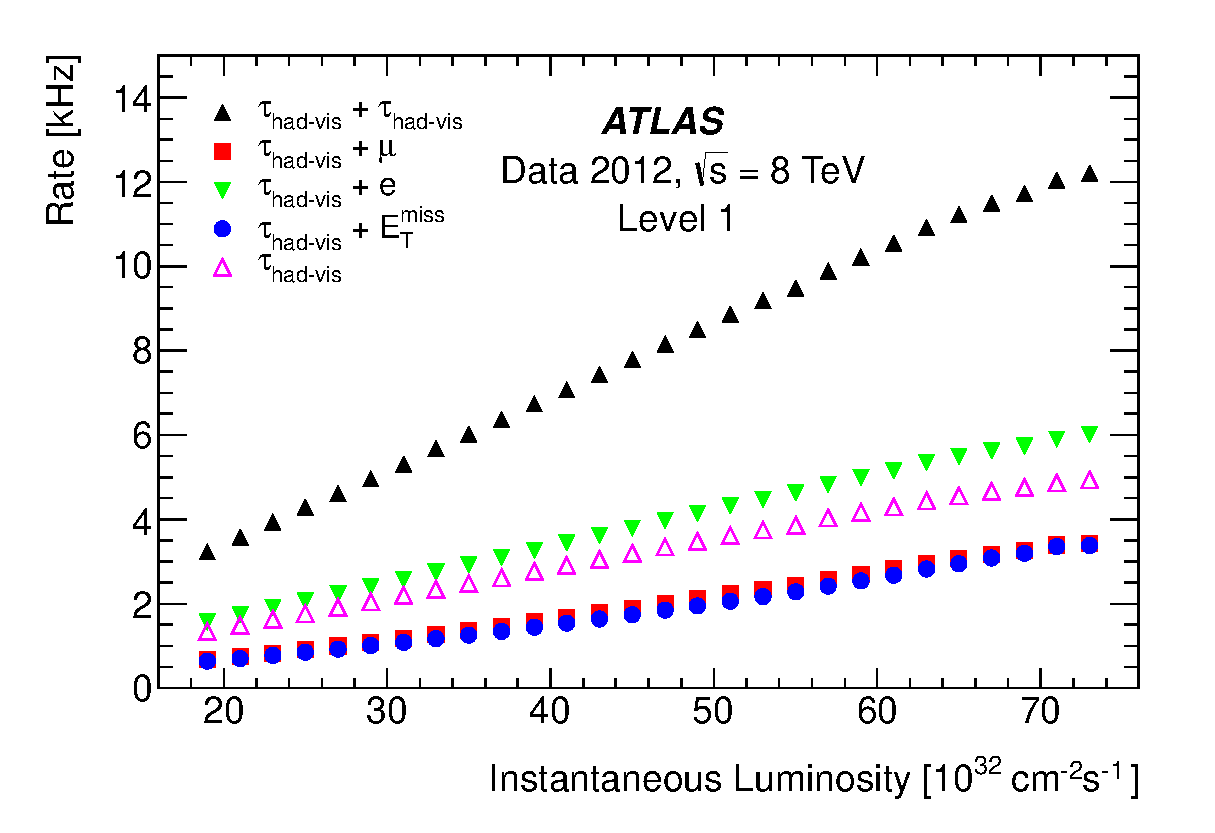
\includegraphics[width=0.48\textwidth]{figures/PERF-2013-06/fig_01a}
  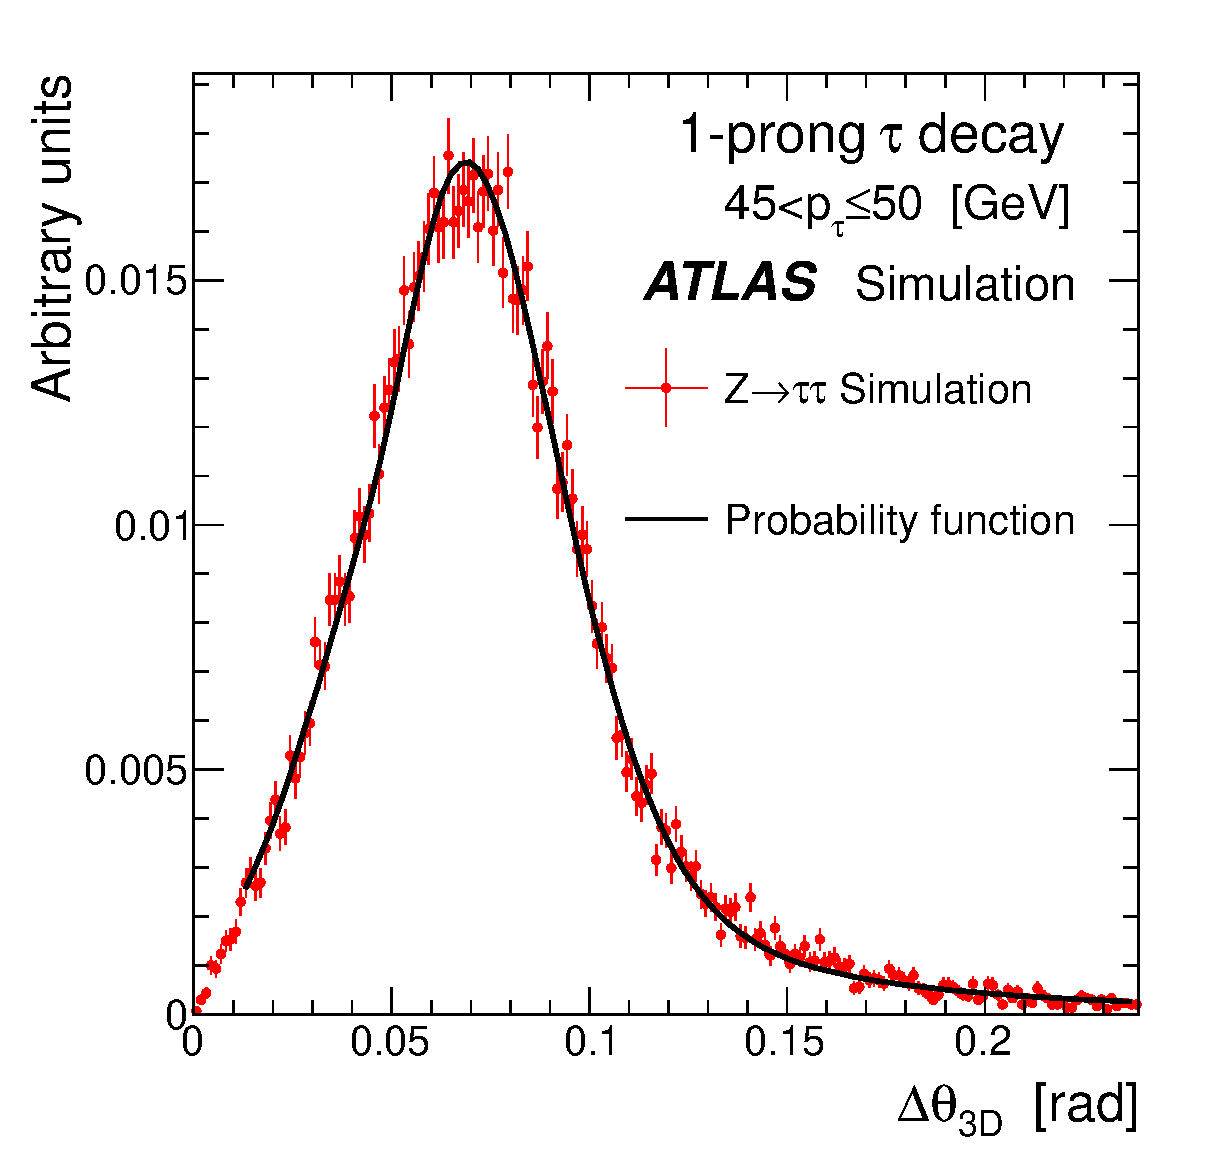
\includegraphics[width=0.48\textwidth]{figures/PERF-2013-06/fig_01b}
  \caption{Variables.}
  \label{fig:prospects-tautriggerrates}
\end{figure}

\subsection{Run-I triggers for $\Htautau$}

In Run-I, only the $\Htautauhh$ analysis relied on $\tauh$ triggers for physics. The $\Htautaulh$ used single lepton triggers with an offline threshold of 26 GeV. $\ell+\tauh$ triggers were considered but ultimately dropped because they brought additional complication to the analysis without significant improvement in sensitivity. The $\Htautaull$ analysis relied on single and di-lepton triggers. The list of triggers used in 2012 data-taking, and their expected 2015 versions, is shown in \cref{tab:prospects-triggersL1} and \cref{tab:prospects-triggersHLT}.

\begin{table}[bp] 
  \centering
  \begin{tabular}{c|c|c}
  channel      & L1, 2012                    & L1, 2015 \\
  \hline\hline
  $\Htautauhh$ & \texttt{2TAU11I\_TAU15}     & no di-$\tauh$ item planned  \\
  \hline
  $\Htautaueh$ & \texttt{EM18VH}             & \texttt{EM24VHI}            \\
%               & \texttt{2TAU11I\_EM14VH}    & \texttt{TAU40\_EM15VHI}     \\
  $\Htautaumh$ & \texttt{MU20}               & \texttt{MU20}               \\
%               & \texttt{TAU8\_MU10}         & \texttt{TAU20I\_MU10}       \\
  \hline
  $\Htautauee$ & \texttt{EM18VH || 2EM10VH}  & \texttt{EM24VHI || 2EM15VH} \\
  $\Htautaumm$ & \texttt{2MU10}              & \texttt{2MU10}              \\
  $\Htautauem$ & \texttt{EM10VH\_MU6}        & \texttt{EM15VH\_MU10}       \\
  \hline\hline
\end{tabular}


  \caption{L1 triggers used in the 2012 $\Htautau$ analysis, and their expected 2015 versions, grouped by $\tautau$ decay channel.}
  \label{tab:prospects-triggersL1}
\end{table}

\begin{table}[bp] 
  \centering
  \begin{tabular}{c|c|c}
  channel      & HLT, 2012                   & HLT, 2015 \\
  \hline\hline
  $\Htautauhh$ & \texttt{tau29Ti\_medium1\_tau20Ti\_medium1} & no di-$\tauh$ item planned \\
  \hline
  $\Htautaueh$ & \texttt{e24vhi\_medium1}                    & \texttt{e28i\_tight}                 \\
%               & \texttt{tau20Ti\_medium1\_e18vh\_medium1}   & \texttt{tau80\_medium\_e18\_medium}  \\
  $\Htautaumh$ & \texttt{mu24i\_tight}                       & \texttt{mu26i\_medium}               \\
%               & \texttt{tau20\_medium1\_mu15}               & \texttt{tau29\_medium\_mu15\_iloose} \\
  \hline
  $\Htautauee$ & \texttt{e24vhi\_medium1 || 2e12Tvh\_loose1} & \texttt{e28i\_tight || 2e17\_loose}  \\
  $\Htautaumm$ & \texttt{mu18\_tight\_mu8\_EFFS}             & \texttt{2mu14}                       \\
  $\Htautauem$ & \texttt{e12Tvh\_medium1\_mu8}               & \texttt{e17\_medium\_mu12}           \\
  \hline\hline
\end{tabular}


  \caption{HLT triggers used in the 2012 $\Htautau$ analysis, and their expected 2015 versions, grouped by $\tautau$ decay channel.}
  \label{tab:prospects-triggersHLT}
\end{table}

\clearpage
\subsection{Run-II triggers}

Trigger options for Run-II are most critical for the $\Htautauhh$ since it relies entirely on $\tauh$ triggers. The $\Htautaull$ analysis will continue to use single and di-lepton triggers, which enjoy low thresholds and are among the most high profile triggers, and thus less likely to be cut in case of unexpectedly high rates. The $\Htautaulh$ analysis will continue to use the single lepton trigger, but the potential benefit of recovering events with leptons below the single lepton trigger thresholds could be helpful. Accordingly, only the $\Htautauhh$ and $\Htautaulh$ analyses were considered for trigger optimizations, with emphasis on $\Htautauhh$.

\subsubsection{Object thresholds}

The first option was to raise object thresholds in the trigger. Given the success of the Run-I analysis, which only included event topologies with additional jets, triggering on one or two additional jets in the event was considered. To assess the impact of this, the Run-I analysis was re-run but with progressively higher thresholds on the final state objects, and the resulting sensitivity was derived. This is shown in \cref{fig:prospects-trigger-evolution}.

\begin{figure}[!htpb]
  \centering
  \includegraphics[width=0.48\textwidth]{figures/trigger/evolution_hadhad}
  \includegraphics[width=0.48\textwidth]{figures/trigger/evolution_lephad}
  \caption{Variables.}
  \label{fig:prospects-trigger-evolution}
\end{figure}

For both $\Htautauhh$ and $\Htautaulh$, triggering on the lead jet in the VBF category was promising, and triggering on the sub-lead jet was not. This configuration would also spare the boosted category from requiring a second jet, which would be inefficient. An offline threshold of $\approx\! 70$ GeV for the lead jet, which corresponds to a L1 threshold of $\approx\! 25$ GeV, did not cost significant sensitivity.

For $\Htautauhh$, raising the threshold on the lead $\tauh$ was more promising then raising the threshold on the sub-lead $\tauh$. For $\Htautaulh$, raising the threshold on the $\tauh$ was more promising than raising the threshold on the lepton.

\subsubsection{L1topo}

A new feature of the L1 trigger in 2015 is the ability to make topological selections, whereas in Run-I, only object multiplicity selections could be made. This topological selection are implemented via the new \texttt{L1topo} processor.

At L1, the dominant background for $\tauh$ triggers is QCD di-jet production. Topological selections can be used in various ways to suppress this process, especially in the $\Htautau$ analysis signal regions where the $\tau\tau$ system tends to be boosted.
%
\begin{description}
    \item[$\Delta\phi(\tau\tau) < X$:] \hfill \\
      QCD di-jets tend to be produced back-to-back in the transverse plane, and the $\tau\tau$ system is usually not due to transverse boost.
    \item[$\Delta\eta(\tau\tau) < X$:] \hfill \\
      QCD di-jets tend to be produced broadly in $\eta$, and the $\tautau$ system tends to have smaller $\Delta\eta$ due to longitudal boost of the $Z/H$.
    \item[$\Delta R(\tau\tau) < X$:] \hfill \\
      This combines discriminating power of $\Delta\phi(\tau\tau)$ and $\Delta\eta(\tau\tau)$.
    \item[$\pt(\tau\tau) > X$:] \hfill \\
      QCD di-jet systems tend to be produced at rest in the transverse plane, and the $\tau\tau$ system is usually not due to transverse boost.
    \item[$\mtautau > X$:] \hfill \\
      QCD di-jet systems tend to be non-resonant and low-$\pt$, and the $\tau\tau$ system is from $Z/H$ decays.
\end{description}
%
The discriminating power of these variables is shown in \cref{fig:prospects-trigger-l1topo}.

\begin{figure}[!htpb]
  \centering
  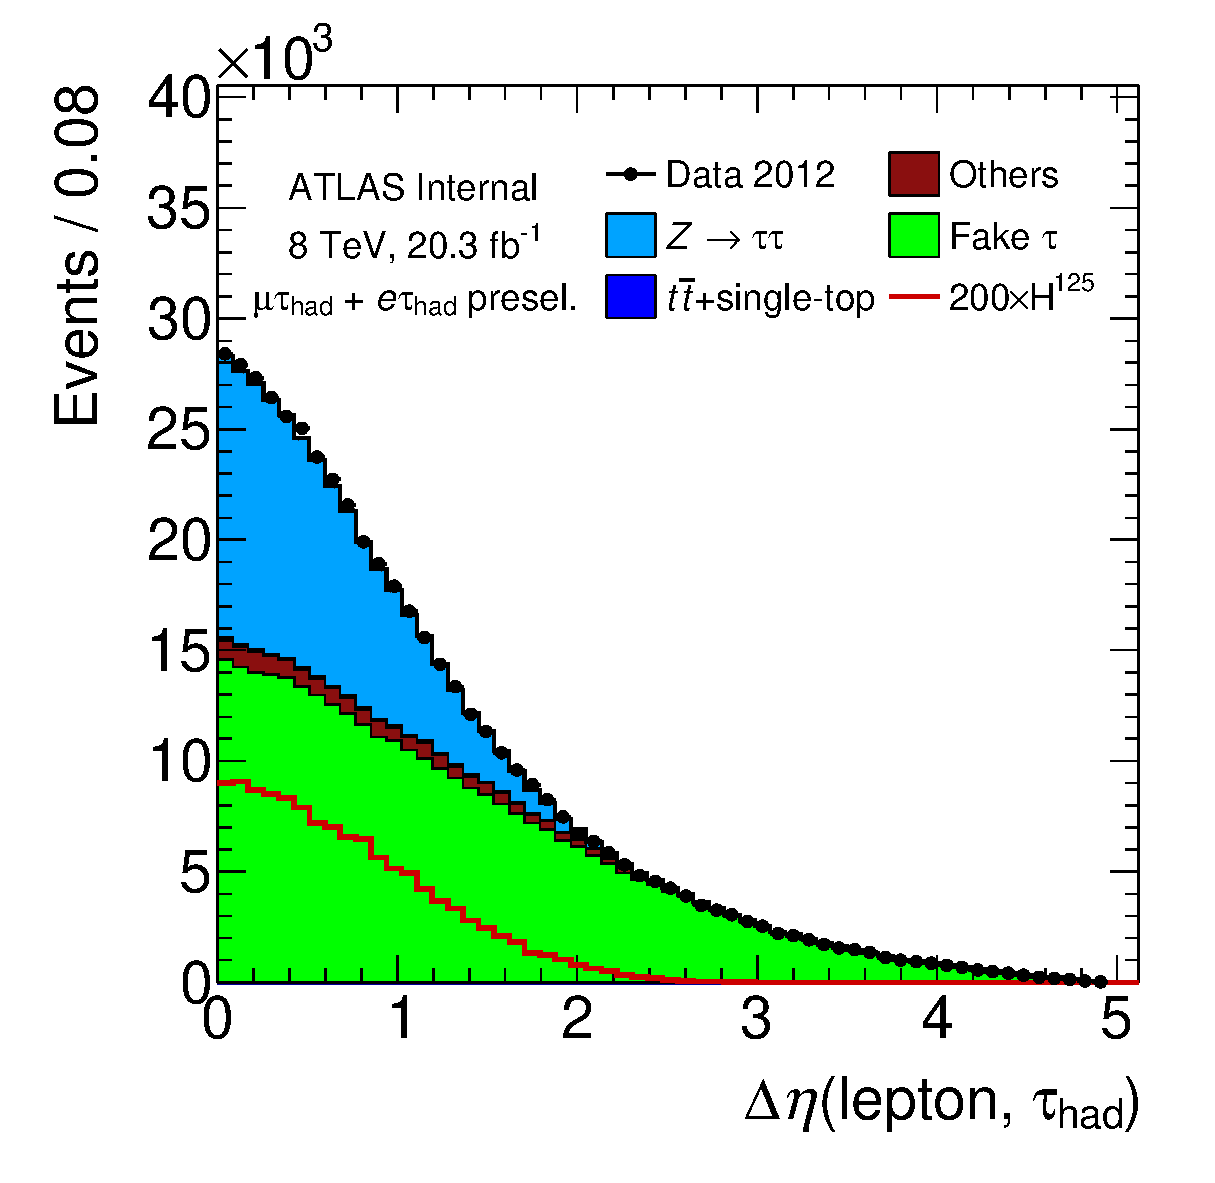
\includegraphics[width=0.32\textwidth]{figures/l1topo/taulep-deta}
  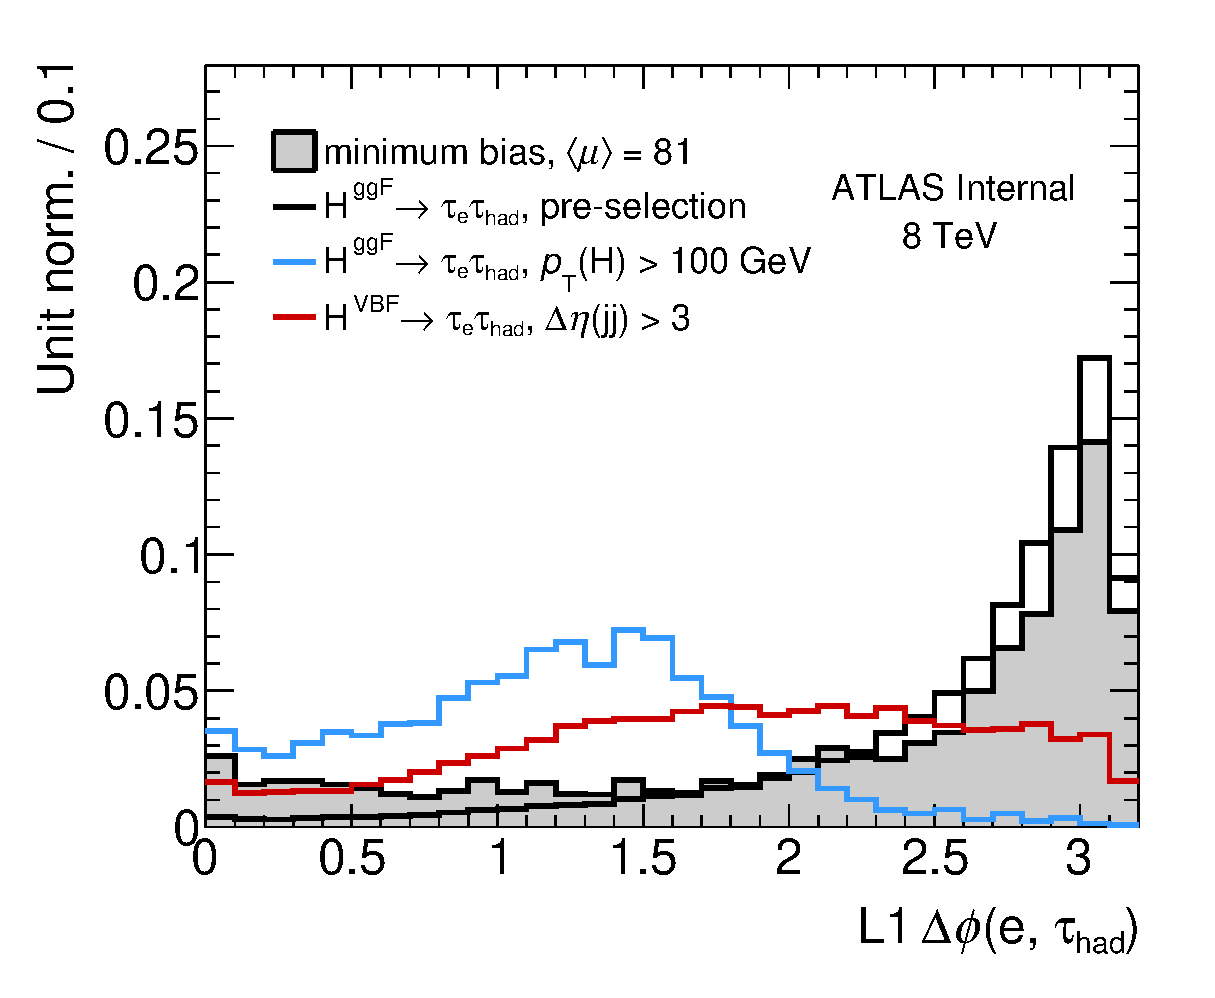
\includegraphics[width=0.32\textwidth]{figures/l1topo/taulep-dphi}
  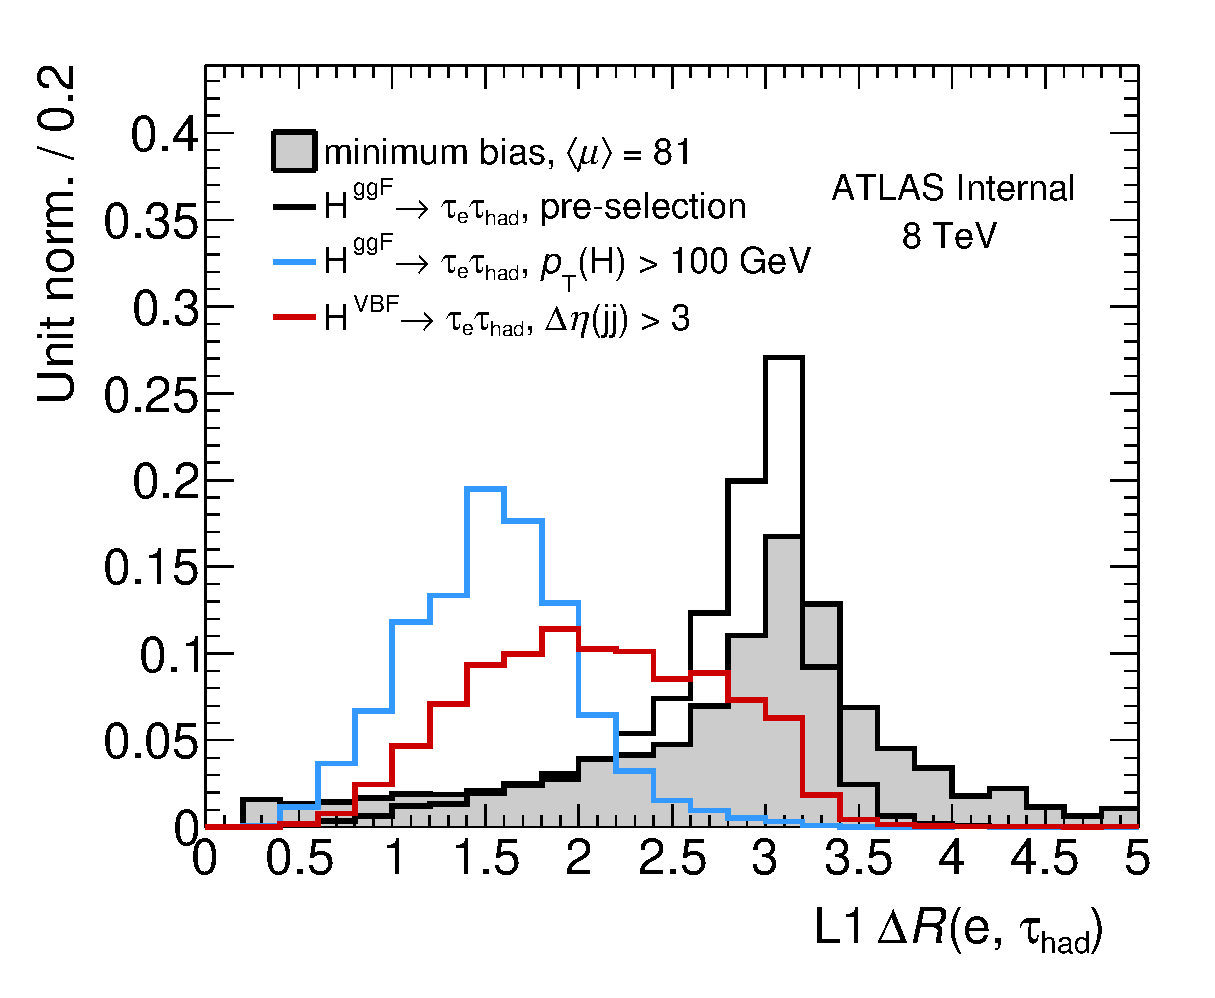
\includegraphics[width=0.32\textwidth]{figures/l1topo/taulep-dR}
  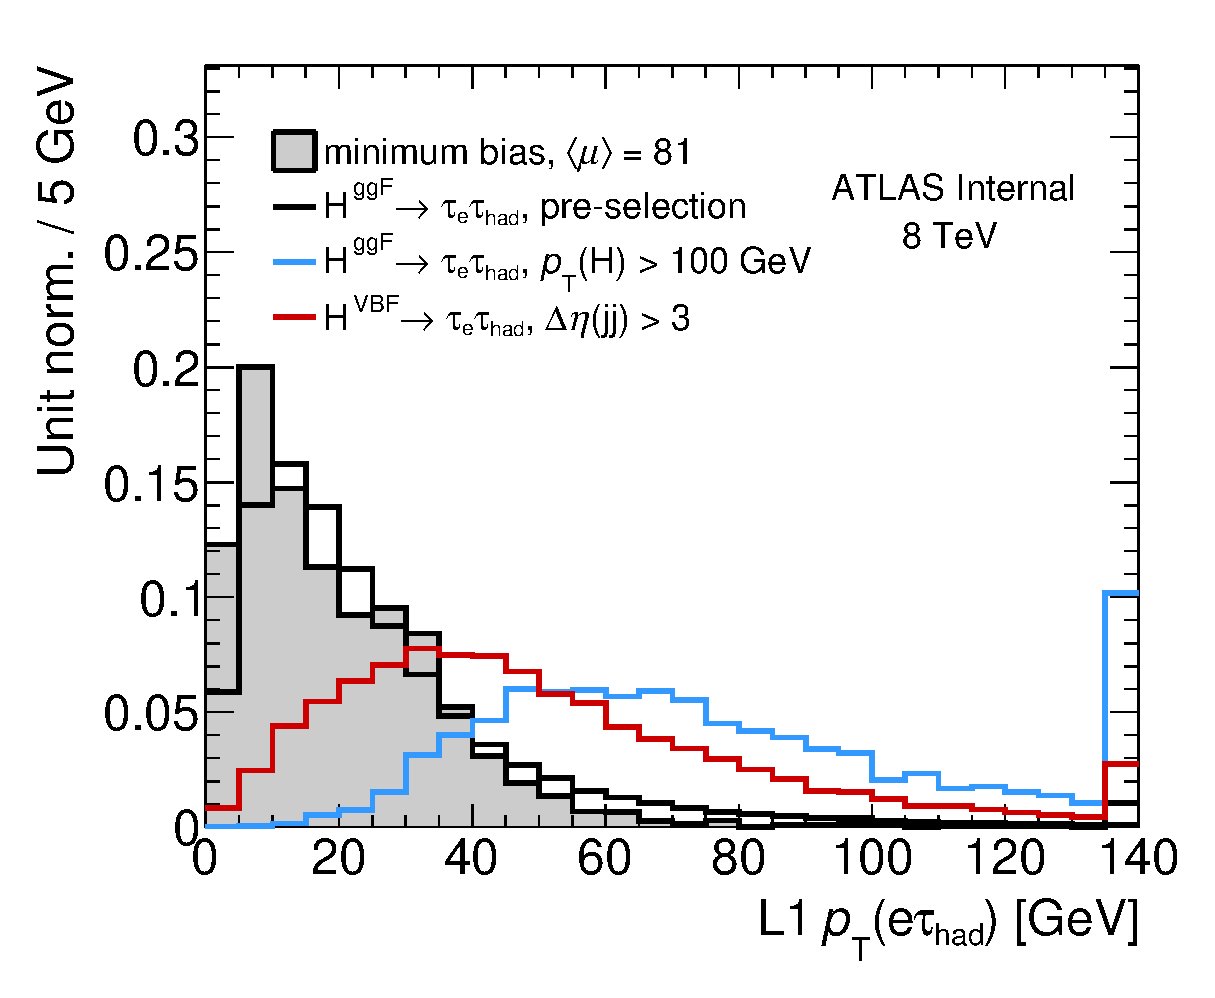
\includegraphics[width=0.32\textwidth]{figures/l1topo/ditau-pt}
  \includegraphics[width=0.32\textwidth]{figures/l1topo/ditau-m}
  \caption{Variables.}
  \label{fig:prospects-trigger-l1topo}
\end{figure}

Of these options, angular discrimination is appealing because the angular resolution for $\tauh$ at L1 is better than momentum resolution, as shown in \cref{fig:prospects-trigger-2011-angular} and \cref{fig:prospects-trigger-resolution}. Sharper efficiency turn-ons can then be expected at HLT and offline. $\Delta R(\tautau) < 2.8$ was ultimately chosen for discrimination because it combines the discriminating power of $\Delta\phi(\tautau)$ and $\Delta\eta(\tautau)$.

The impact of requiring an additional jet and $\Delta R(\tautau) < 2.8$ on the predicted 2015 L1 trigger rate is shown in \cref{tab:prospects-L1rate-evolution}. A ten-fold reduction of the rate is achieved without signicant loss of sensitivity.

\clearpage
\begin{figure}[!htpb]
  \centering
  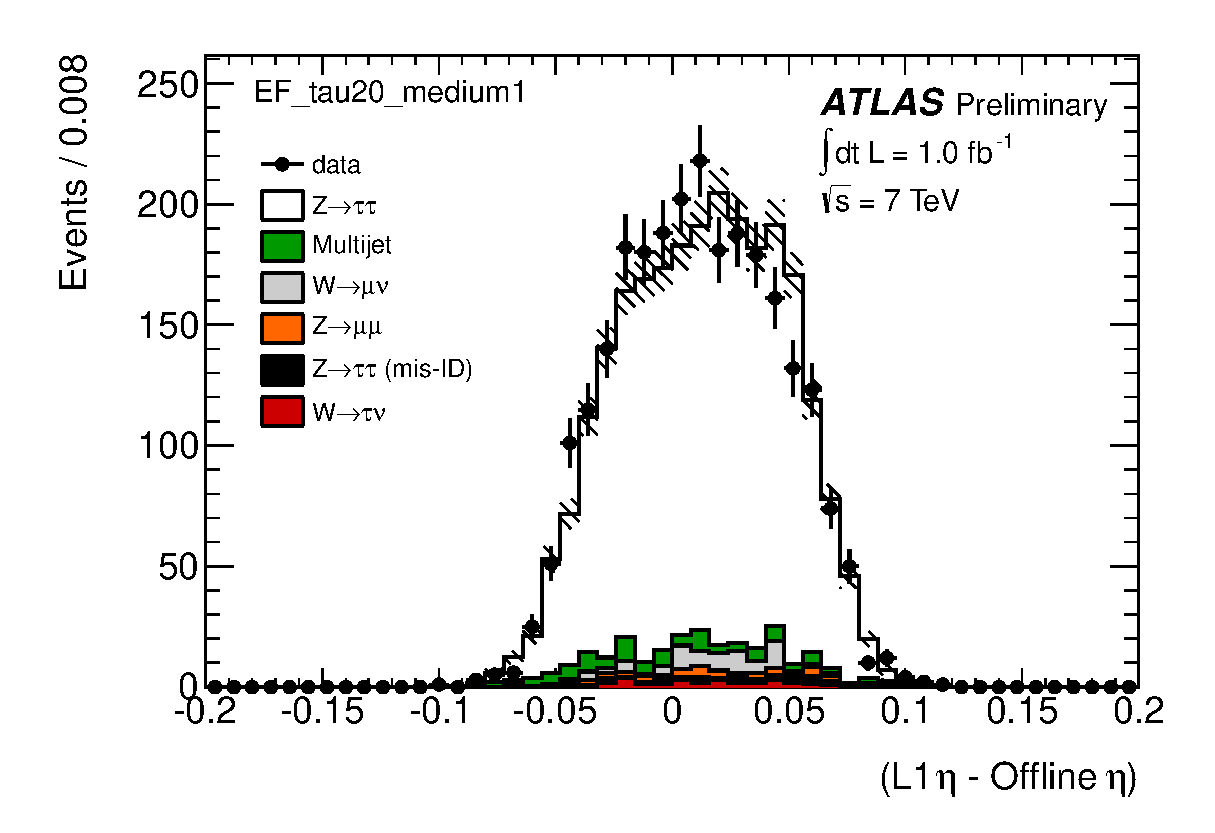
\includegraphics[width=0.48\textwidth]{figures/ATL-COM-DAQ-2012-001/c_L1_etares}
  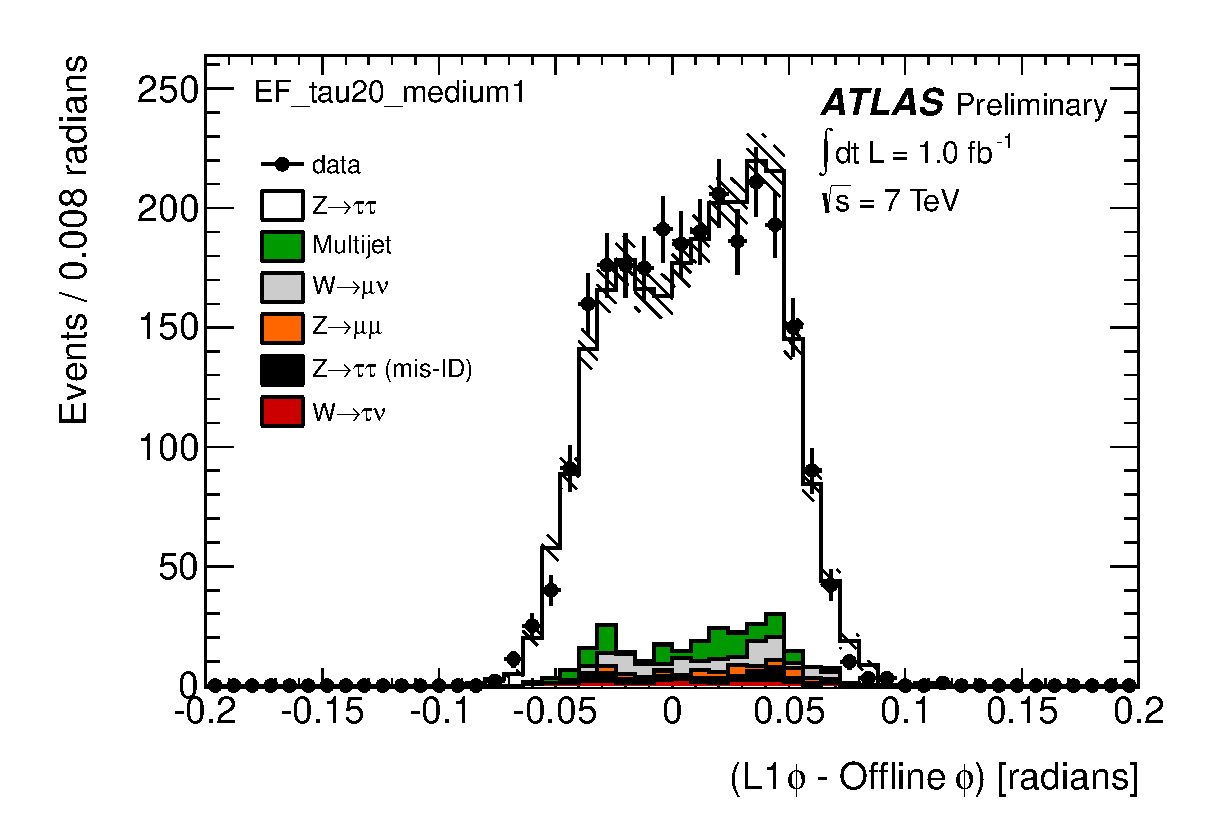
\includegraphics[width=0.48\textwidth]{figures/ATL-COM-DAQ-2012-001/c_L1_phires}
  \caption{Variables.}
  \label{fig:prospects-trigger-2011-angular}
\end{figure}

\begin{figure}[!htpb]
  \centering
  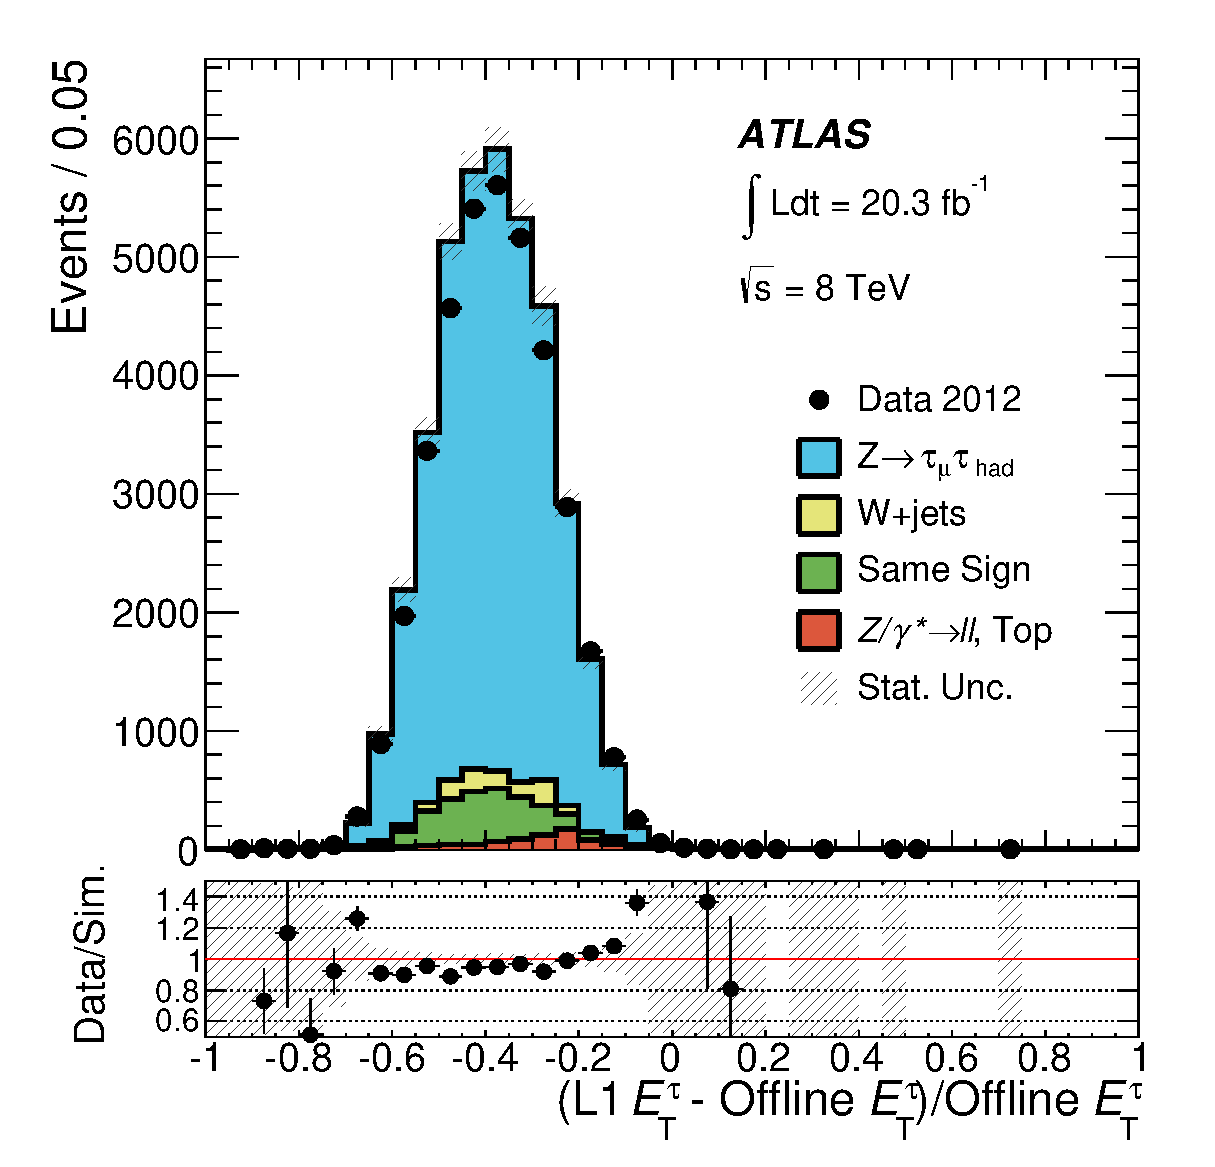
\includegraphics[width=0.48\textwidth]{figures/PERF-2013-06/fig_18a}
  \includegraphics[width=0.48\textwidth]{figures/PERF-2013-06/fig_18c}
  \caption{Variables.}
  \label{fig:prospects-trigger-resolution}
\end{figure}

\begin{table}[!htpb] 
  \centering
  \begin{tabular}{lccc}
  L1 item                 & Rate [kHz] & Unique rate [kHz] & Comment \\
  \hline
  2TAU11                  & 181        & 147               & $\Htauhtauh$, early 2011       \\
  2TAU11I                 & 121        &  99               & $\Htauhtauh$, late 2011        \\
  TAU15I TAU11I           &  96        &  75               & $\Htauhtauh$, 2012             \\
  TAU20I TAU11I           &  69        &  48               & Raise lead $\tauh$ $\pt$     \\
  TAU20I TAU12I           &  61        &  42               & Raise sub-lead $\tauh$ $\pt$ \\
  TAU20I TAU12I J25       &  20        &  12               & Additional jet            \\
  TAU20I TAU12I J25 DR2.8 &   7.8      &   4.3             & $\dRtauhtauh < 2.8$          \\
\end{tabular}


  \caption{L1 trigger items and rate predictions for 2015 data-taking. A baseline L1 menu is used for calculating the unique rate.}
  \label{tab:prospects-L1rate-evolution}
\end{table}
\clearpage

\subsubsection{Sensitivity gain in $\Htautaulh$ with $\ell+\tau_h$ triggers}

To assess the potential gain in sensitivity of $\ell+\tau_h$ triggers in 2015, the $\Htautaulh$ analysis was re-run in the regime below the single lepton trigger threshold. Kinematic distributions are shown in \cref{fig:prospects-ltt-taus} and \cref{fig:prospects-ltt-jets}, including the final BDT discriminant.

Using the $Z_A$ metric, a significant improvement in sensitivity was not observed.

\clearpage
\begin{figure}[tp]
  \centering
  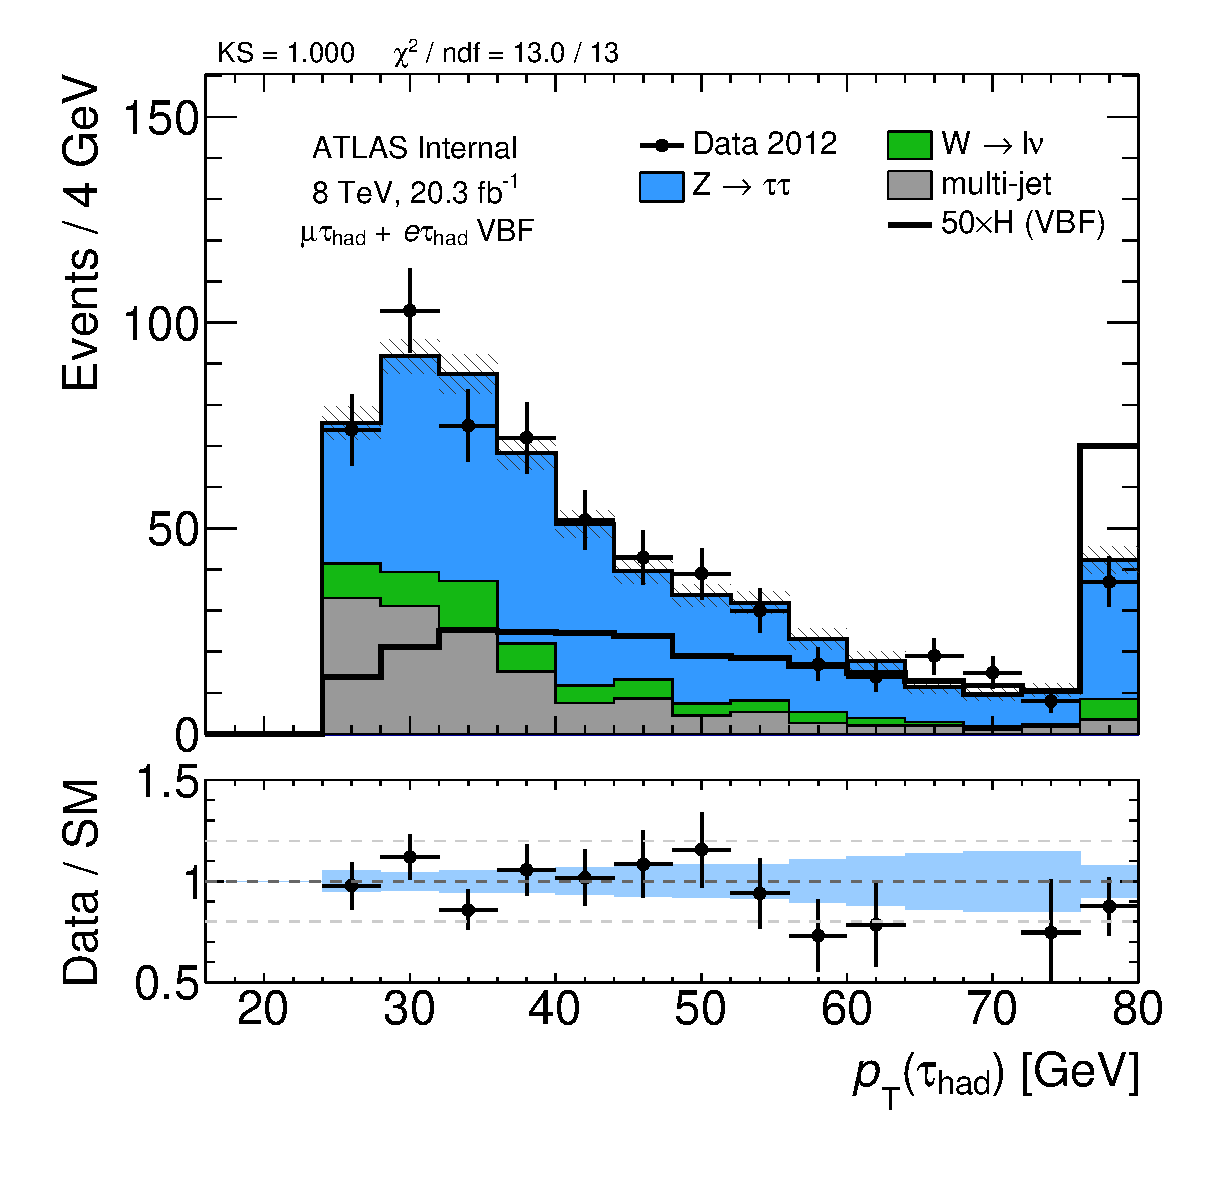
\includegraphics[width=0.32\textwidth]{figures/vbf-LTT/tau-pt}
  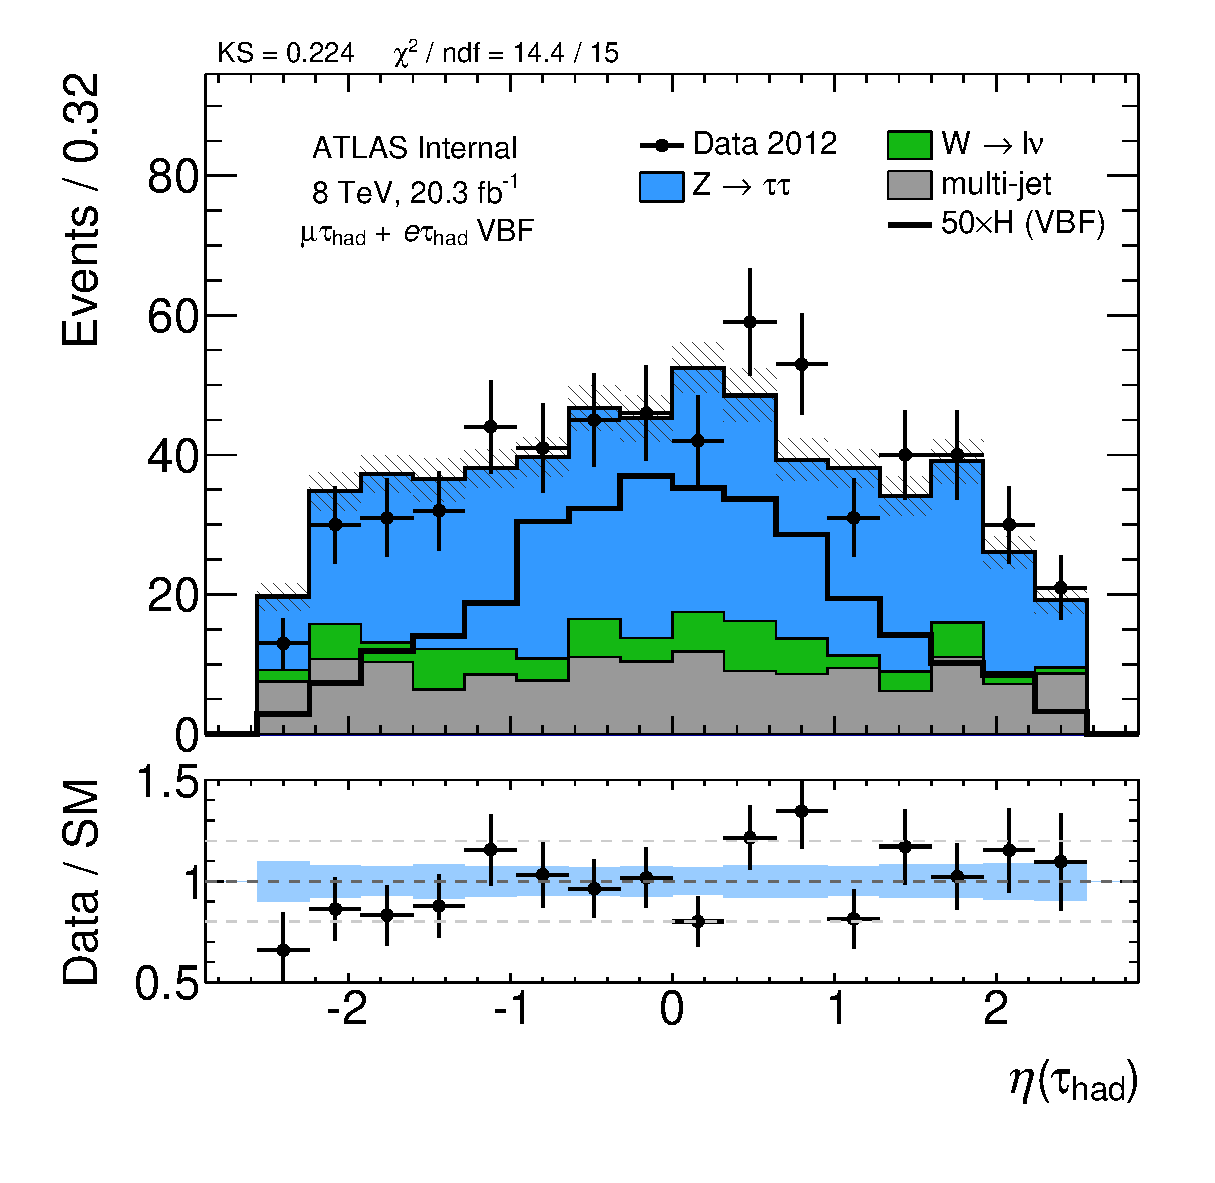
\includegraphics[width=0.32\textwidth]{figures/vbf-LTT/tau-eta}
  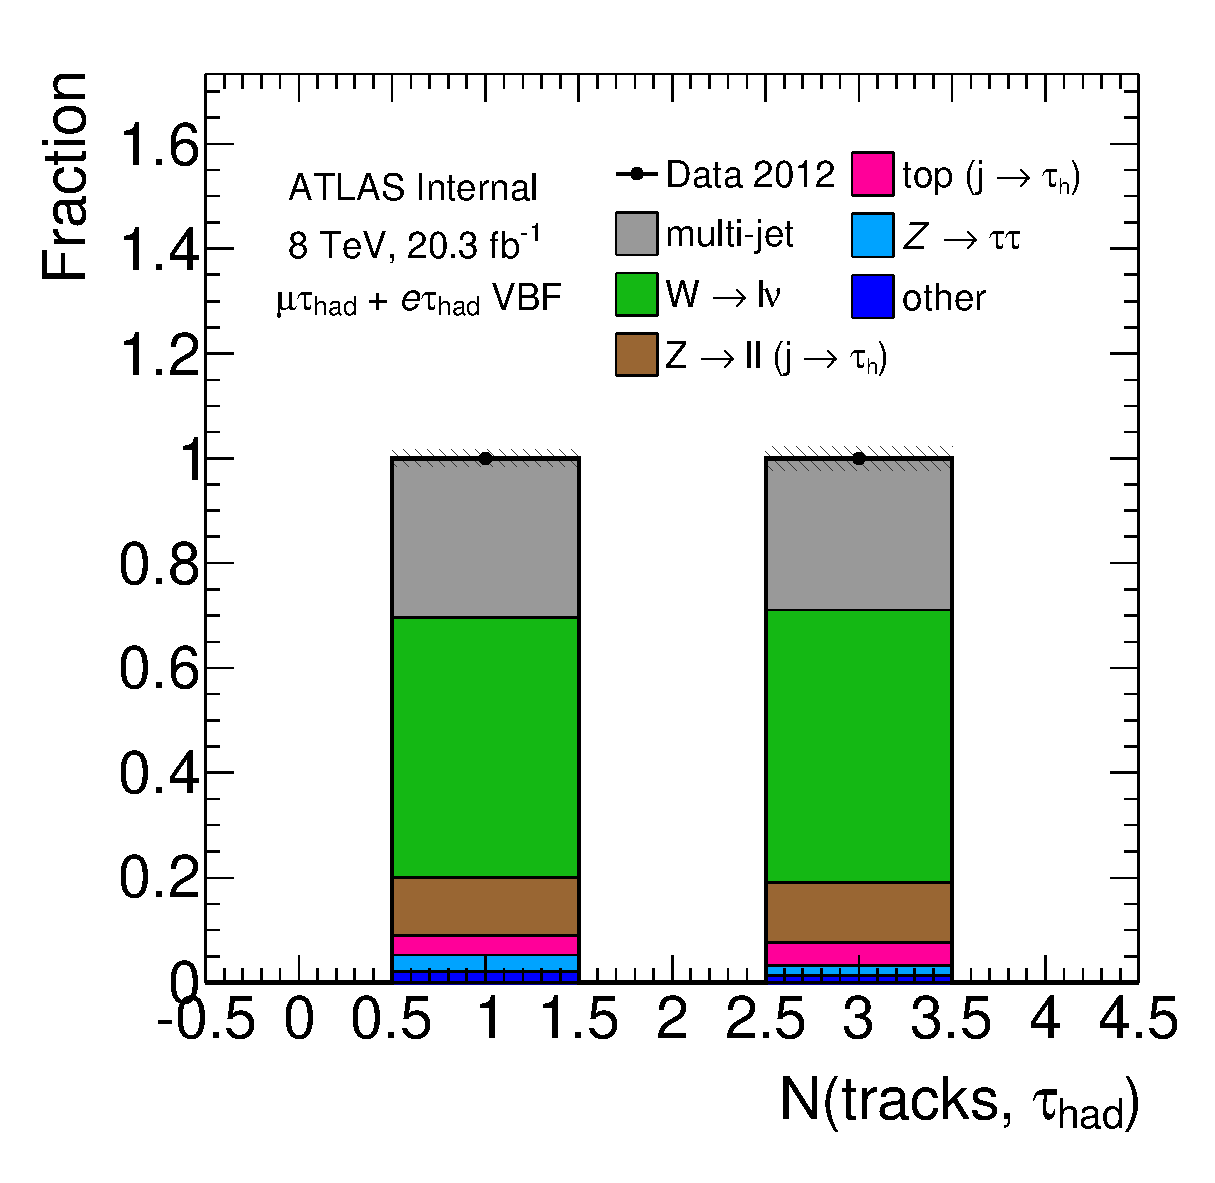
\includegraphics[width=0.32\textwidth]{figures/vbf-LTT/tau-numTrack}
  % --------------
  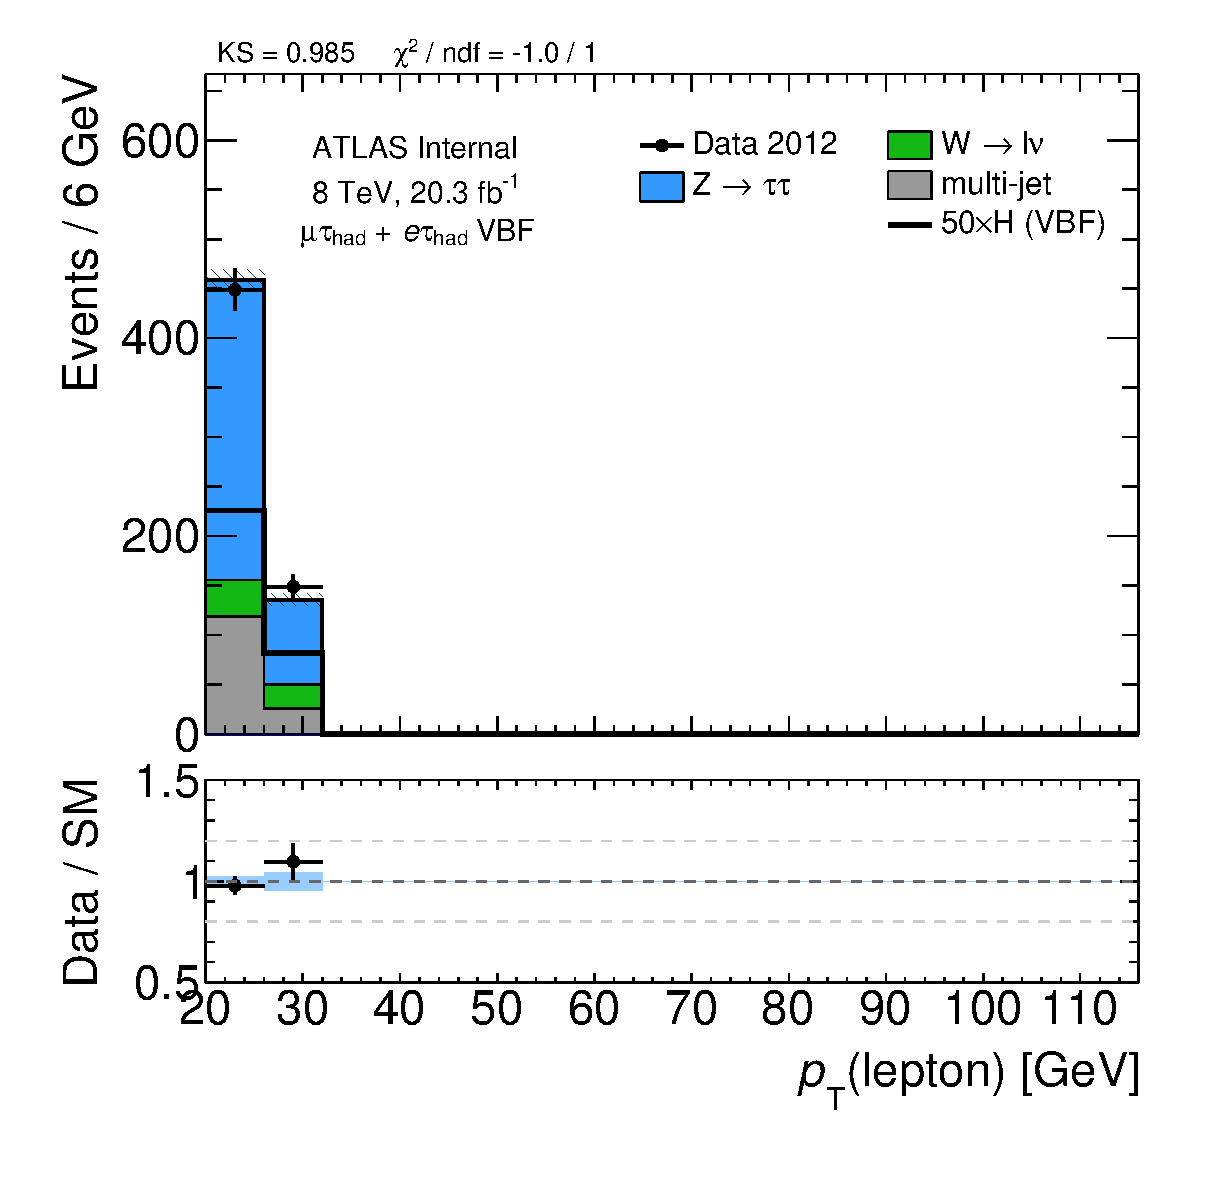
\includegraphics[width=0.32\textwidth]{figures/vbf-LTT/lep-pt-hi}
  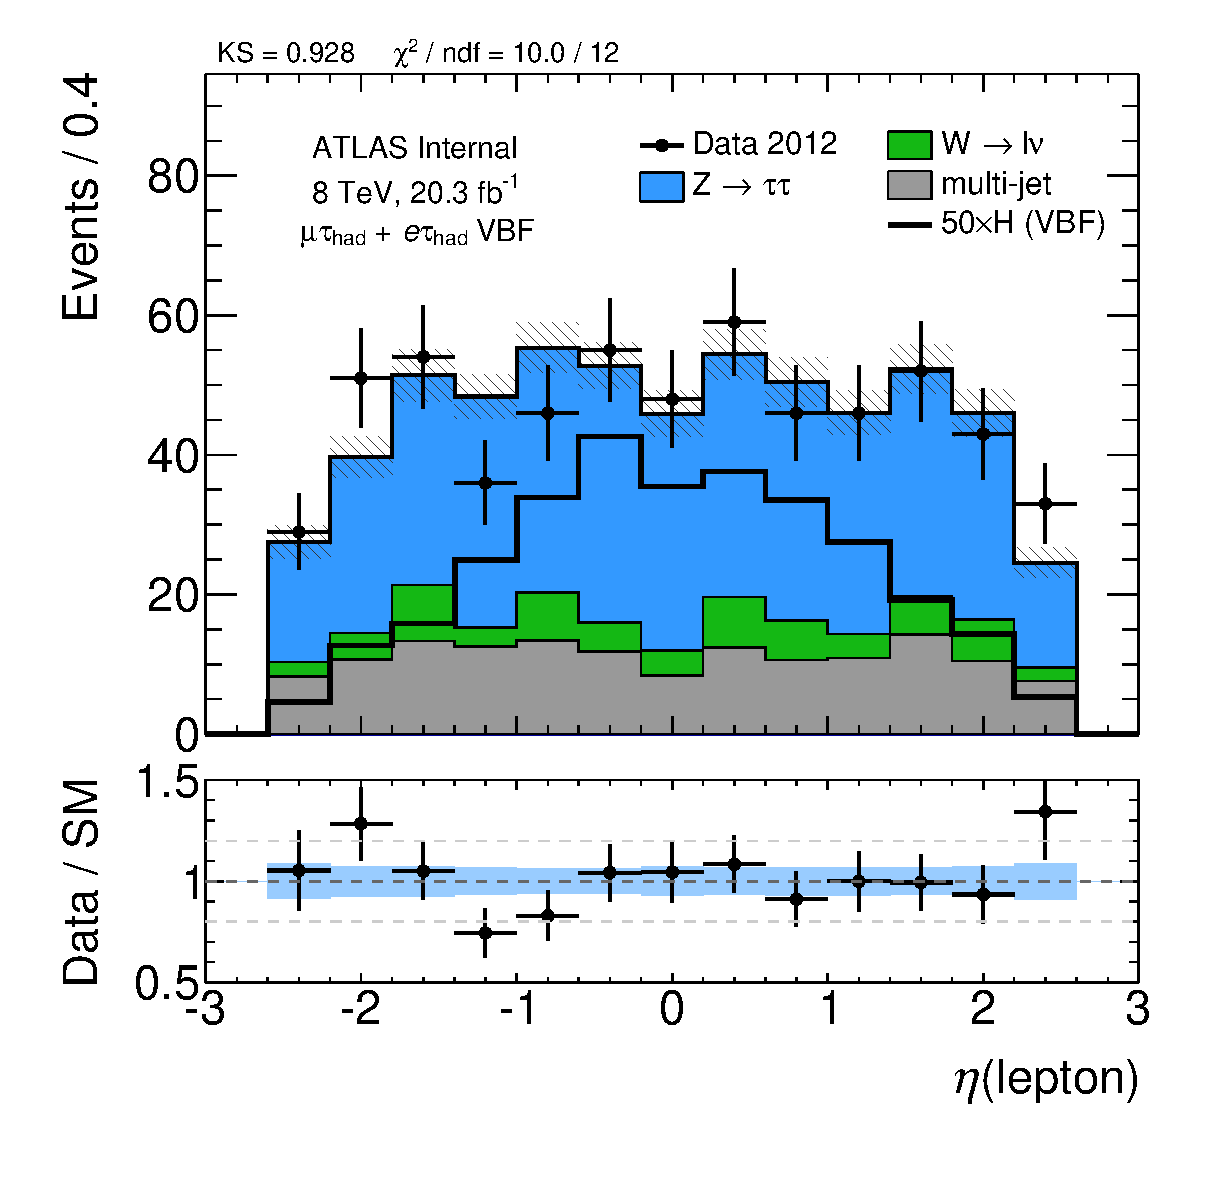
\includegraphics[width=0.32\textwidth]{figures/vbf-LTT/lep-eta}
  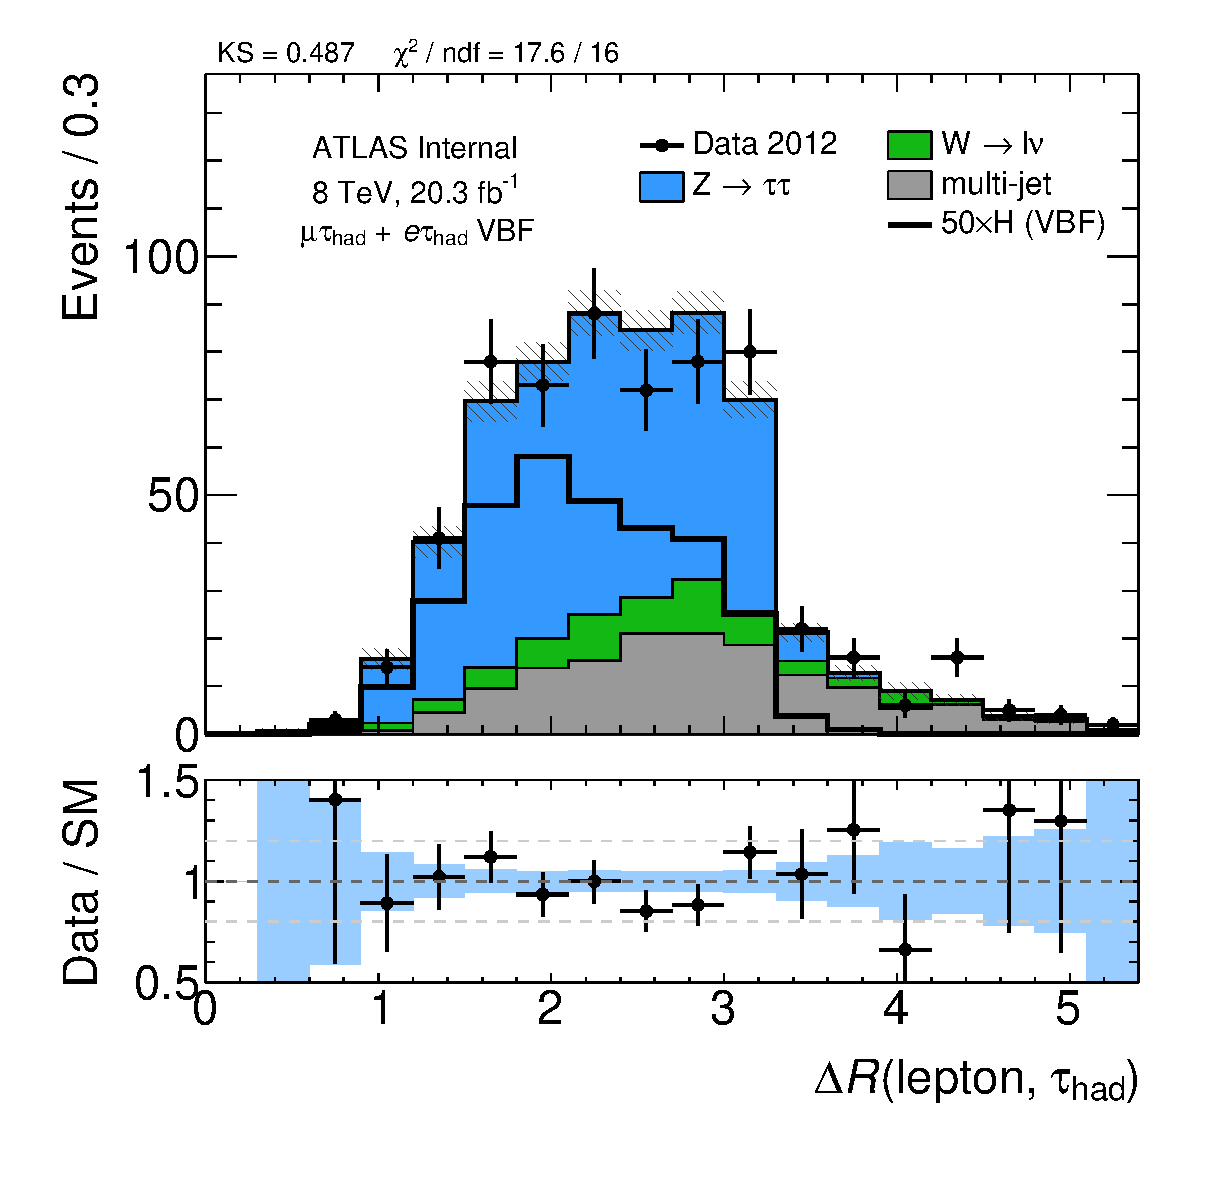
\includegraphics[width=0.32\textwidth]{figures/vbf-LTT/taulep-dR}
  % --------------
  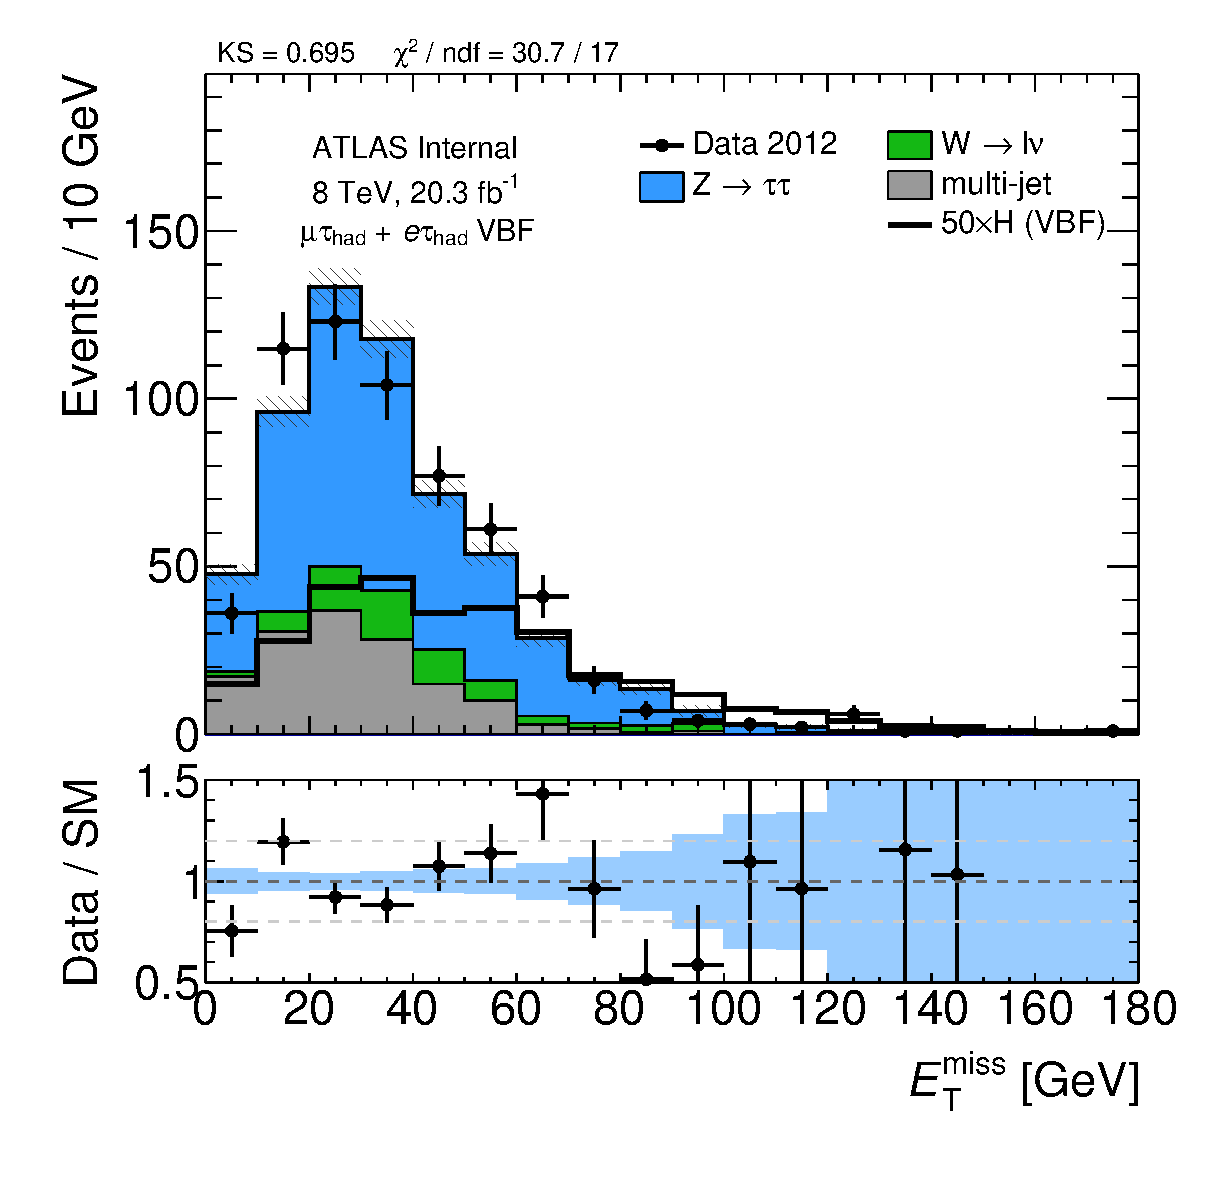
\includegraphics[width=0.32\textwidth]{figures/vbf-LTT/met-pt-hi}
  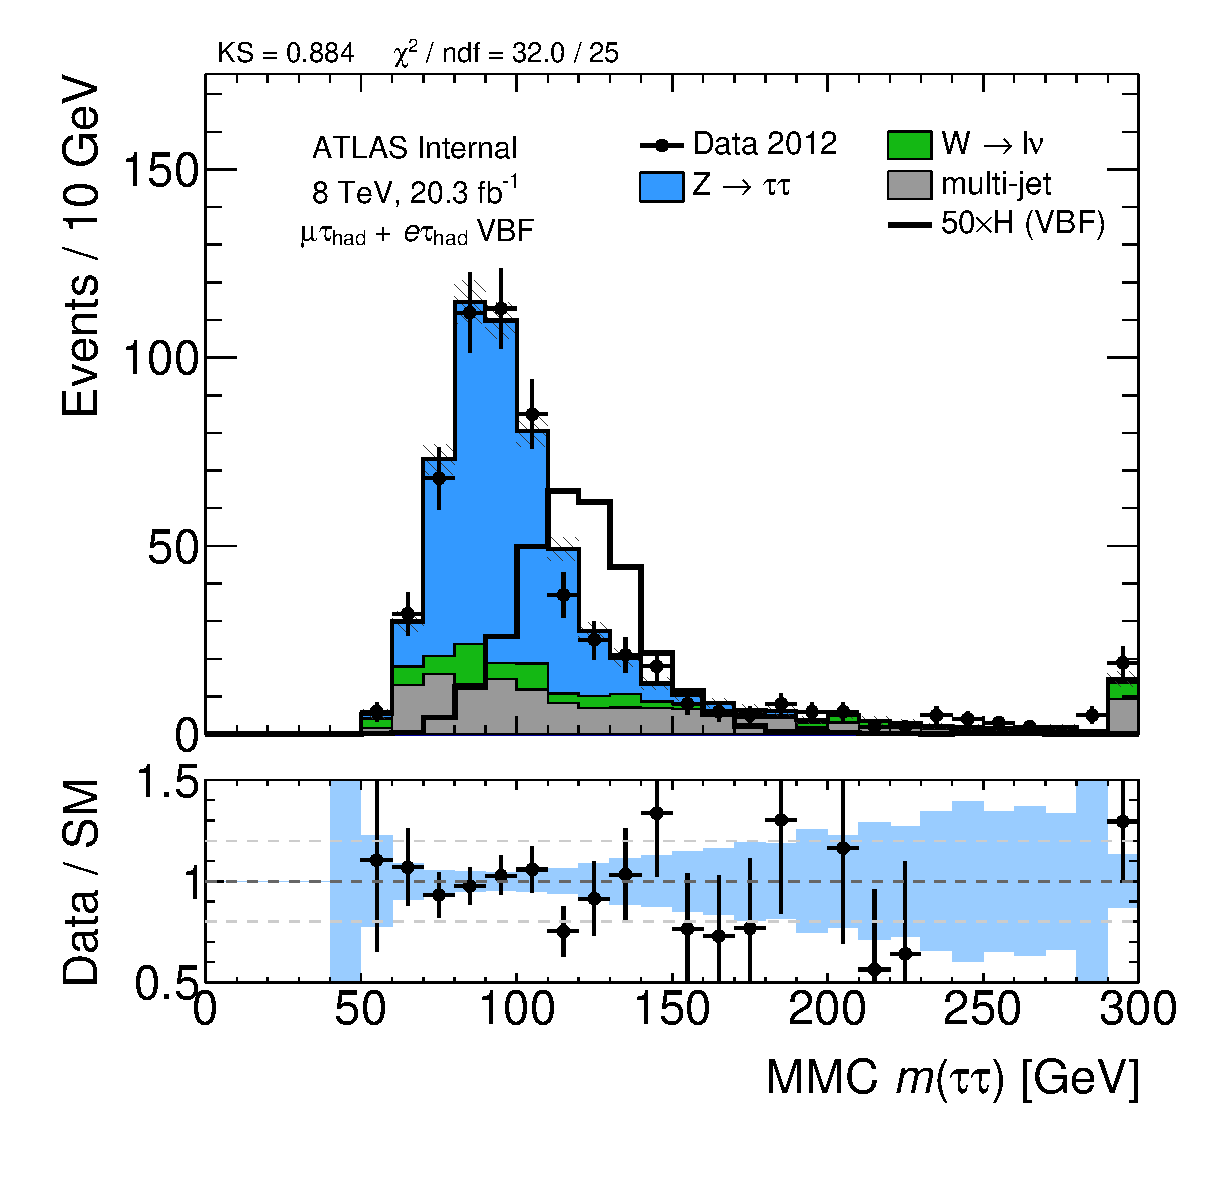
\includegraphics[width=0.32\textwidth]{figures/vbf-LTT/mMMC}
  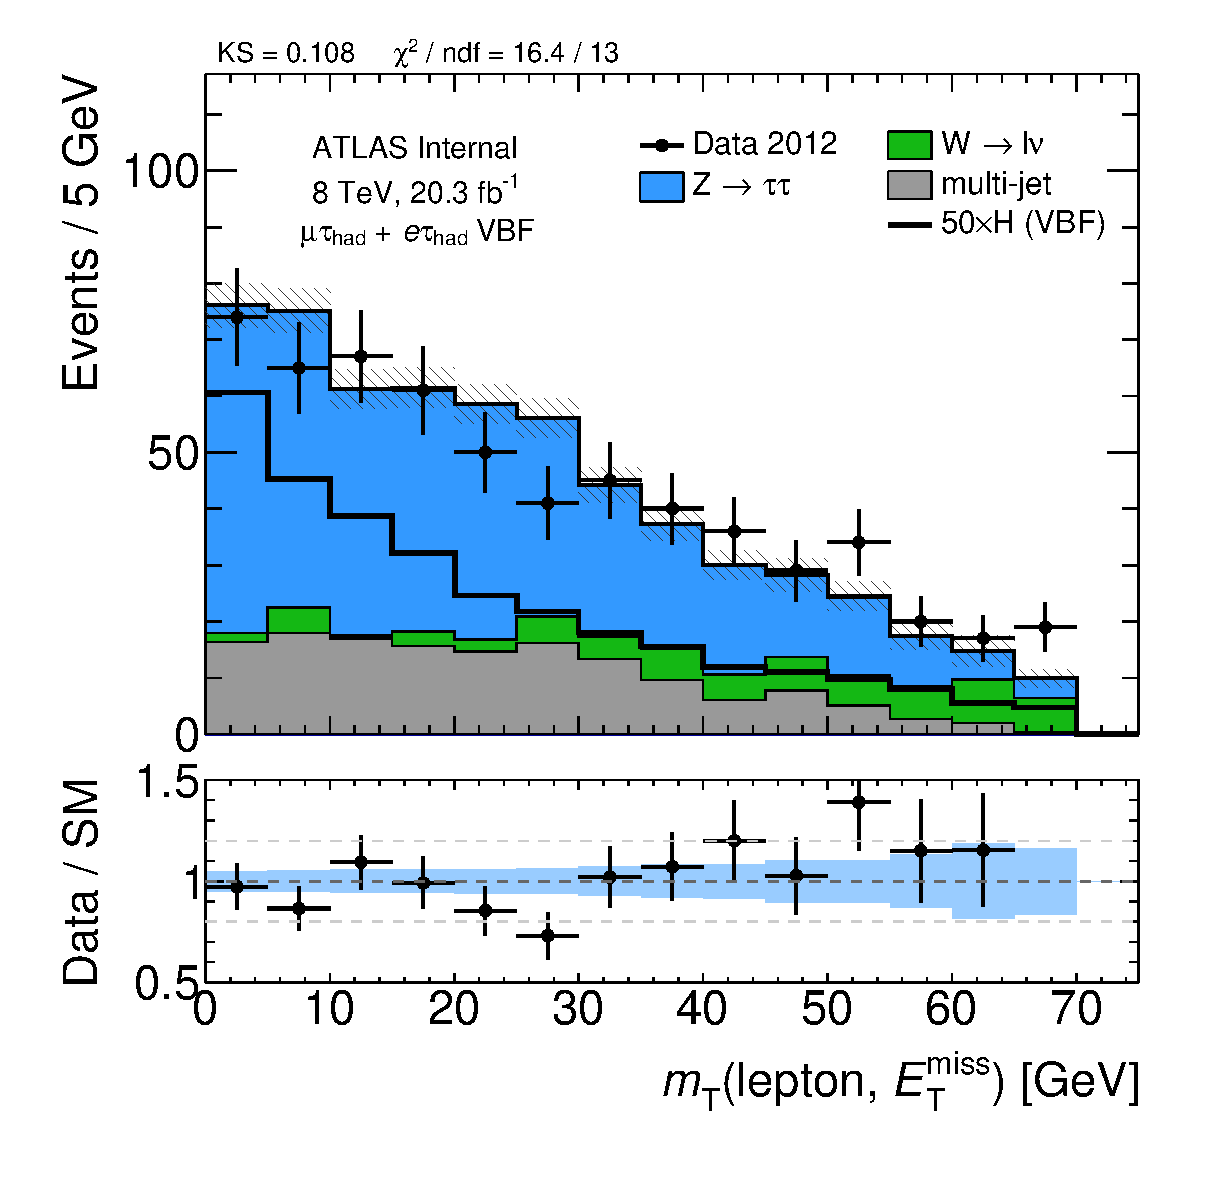
\includegraphics[width=0.32\textwidth]{figures/vbf-LTT/mT}
  % --------------
  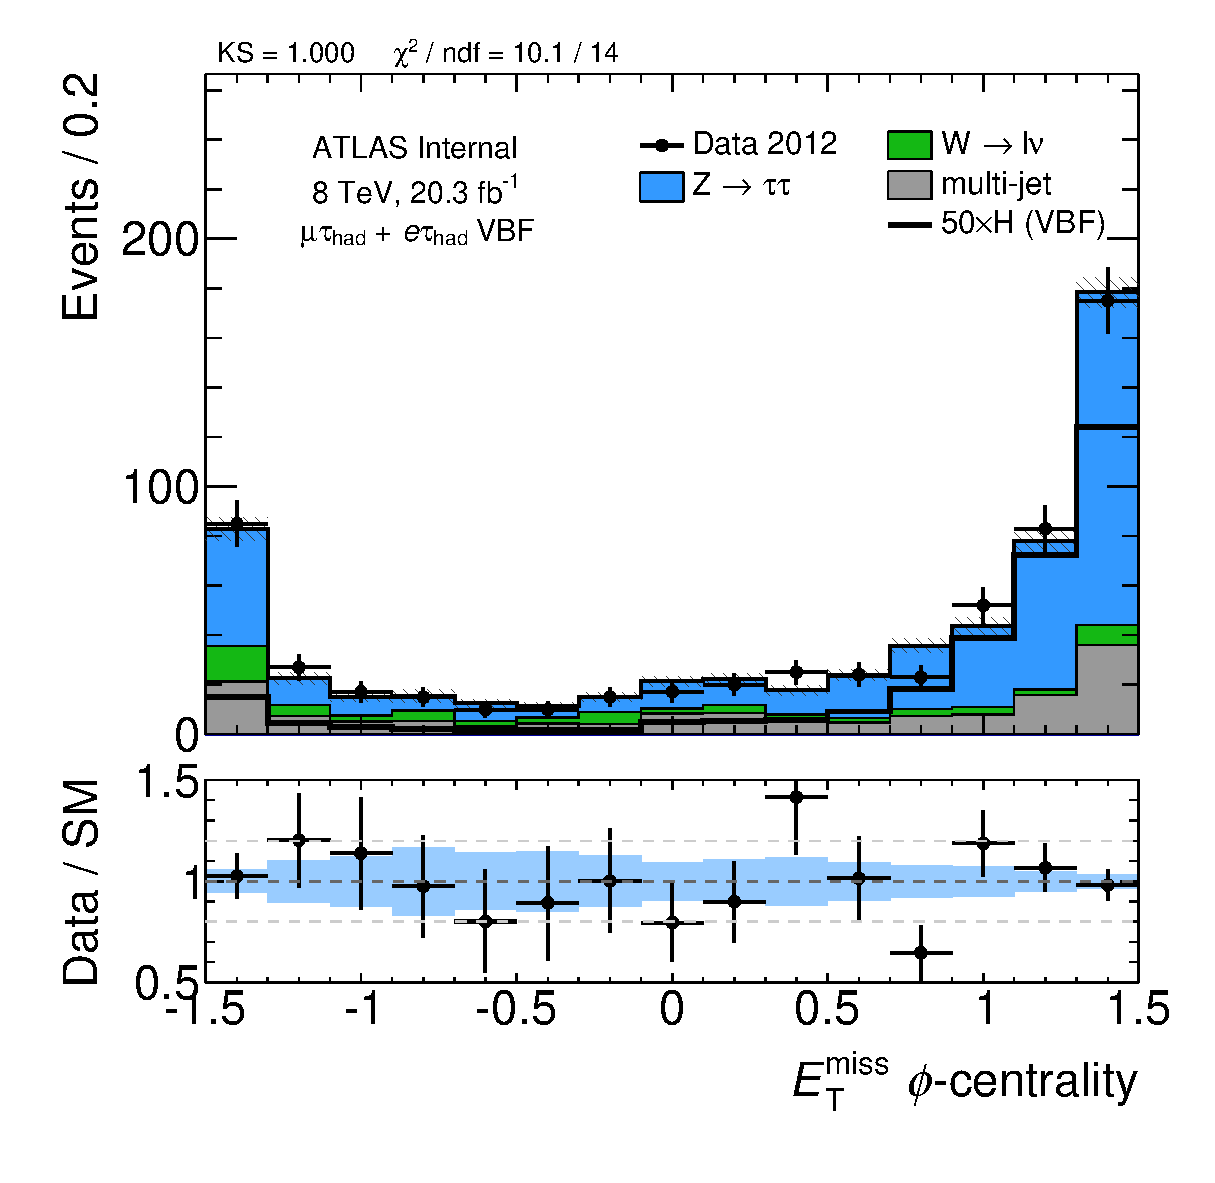
\includegraphics[width=0.32\textwidth]{figures/vbf-LTT/met-phi-centrality}
  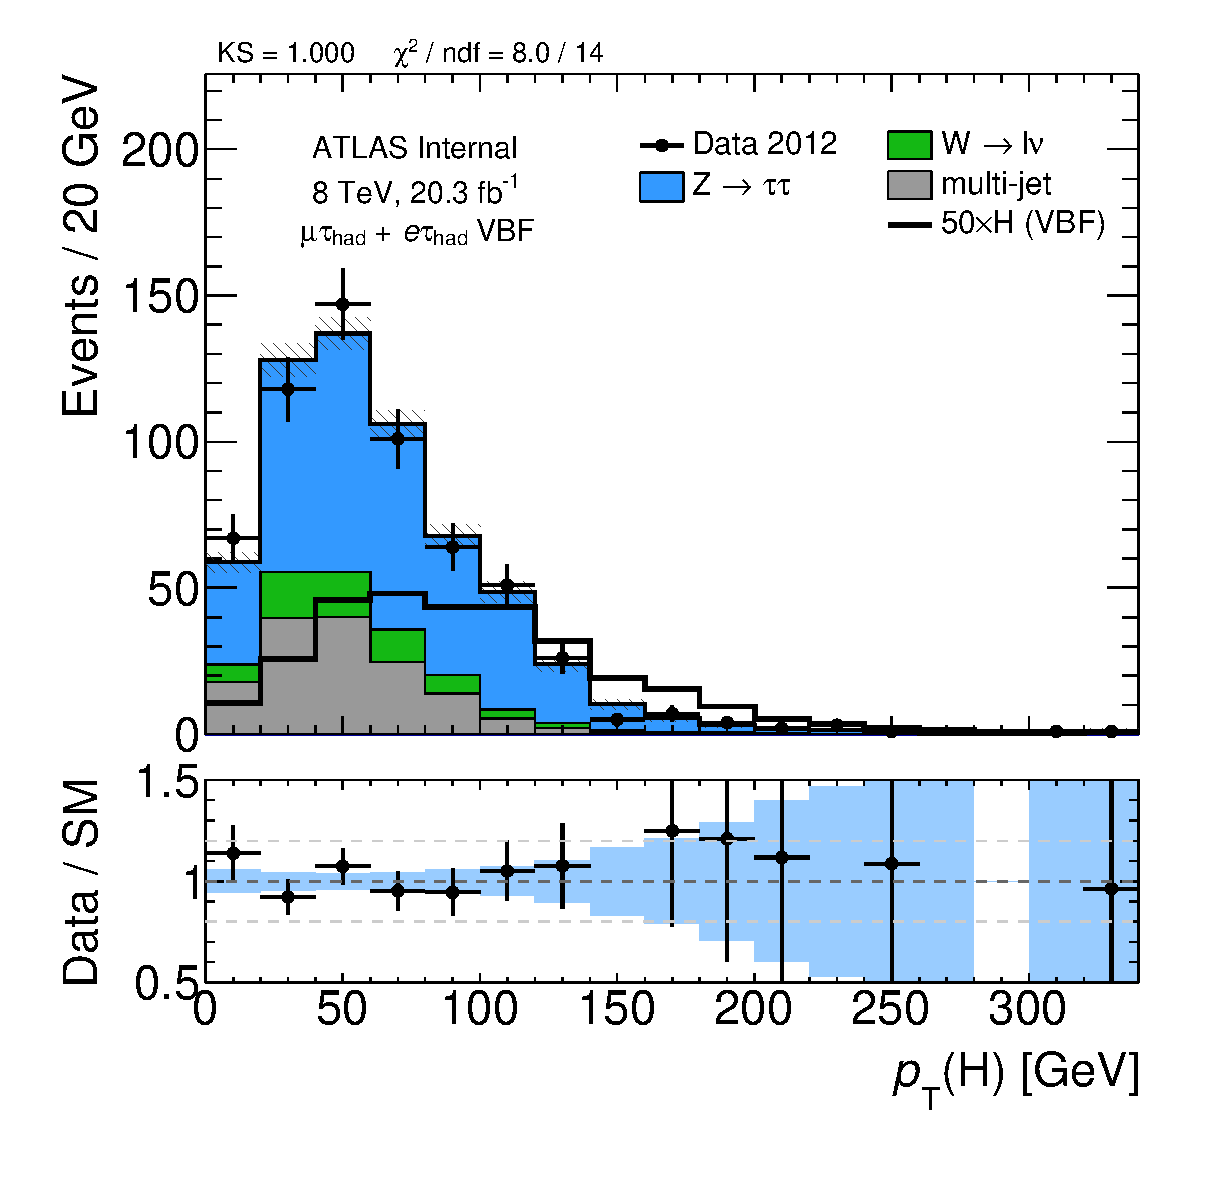
\includegraphics[width=0.32\textwidth]{figures/vbf-LTT/H-pt-hi}
  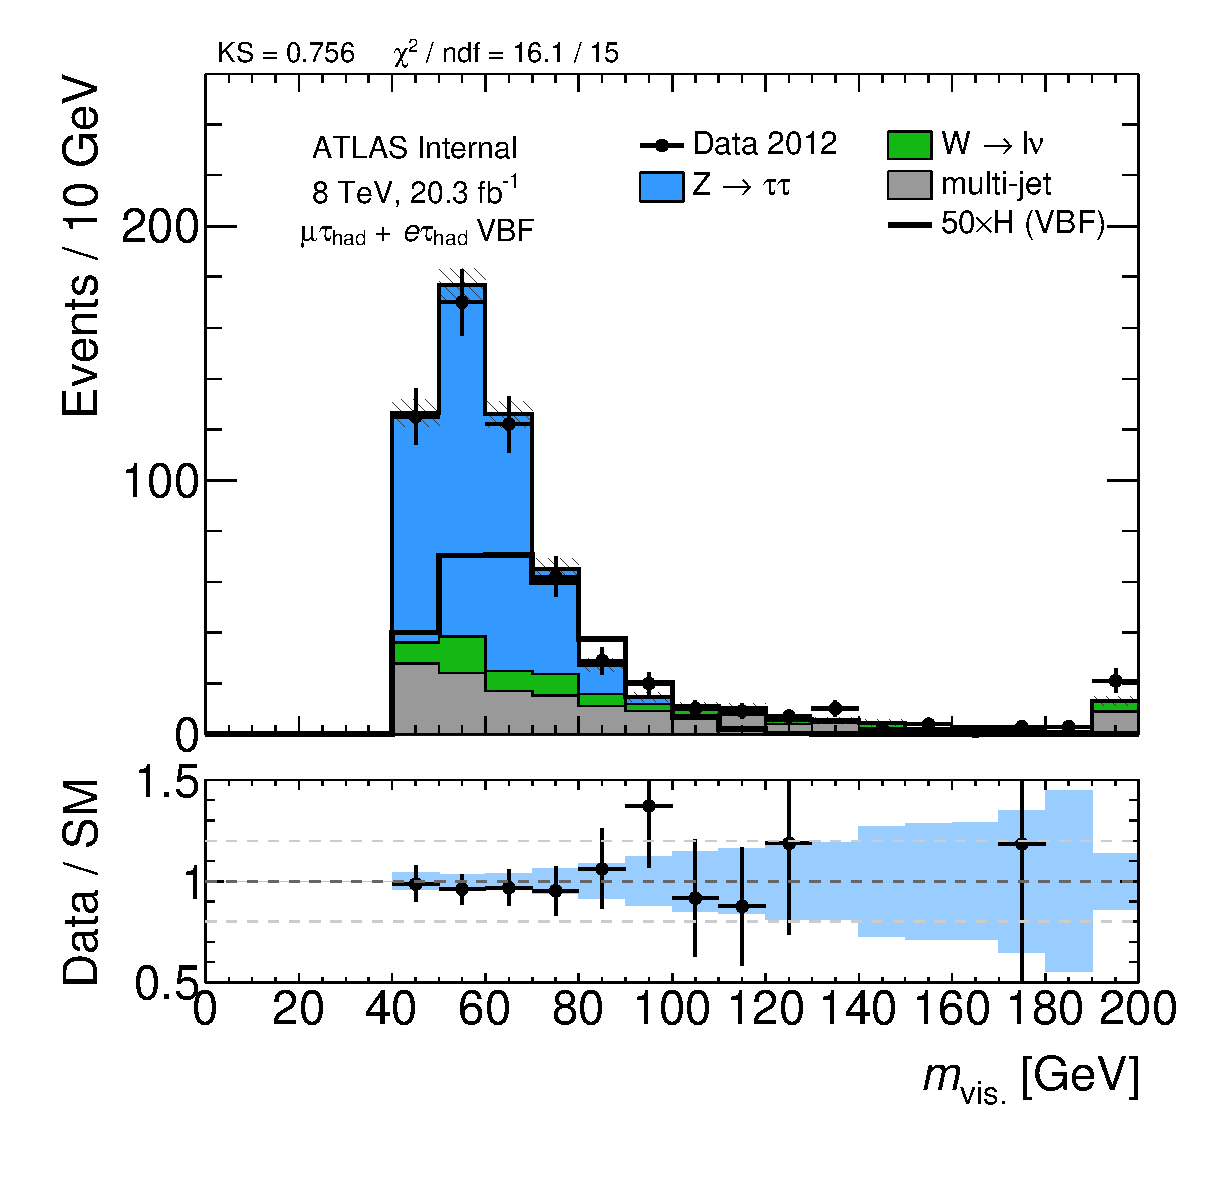
\includegraphics[width=0.32\textwidth]{figures/vbf-LTT/mvis}
  \caption{Variables.}
  \label{fig:prospects-ltt-taus}
\end{figure}

\clearpage
\begin{figure}[tp]
  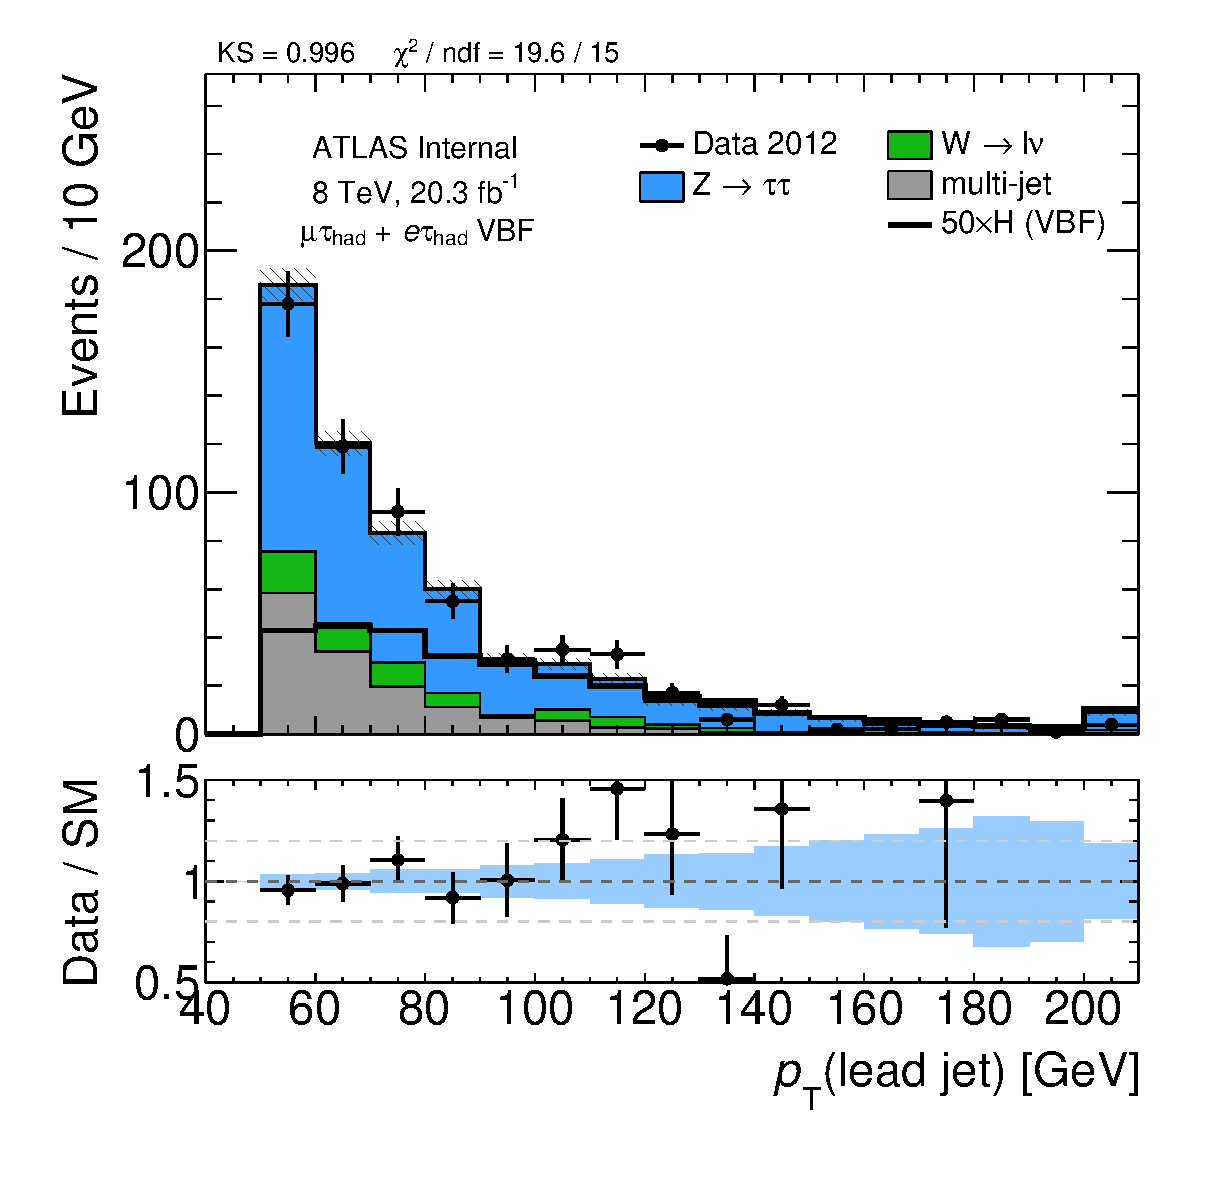
\includegraphics[width=0.32\textwidth]{figures/vbf-LTT/jet-1-pt}
  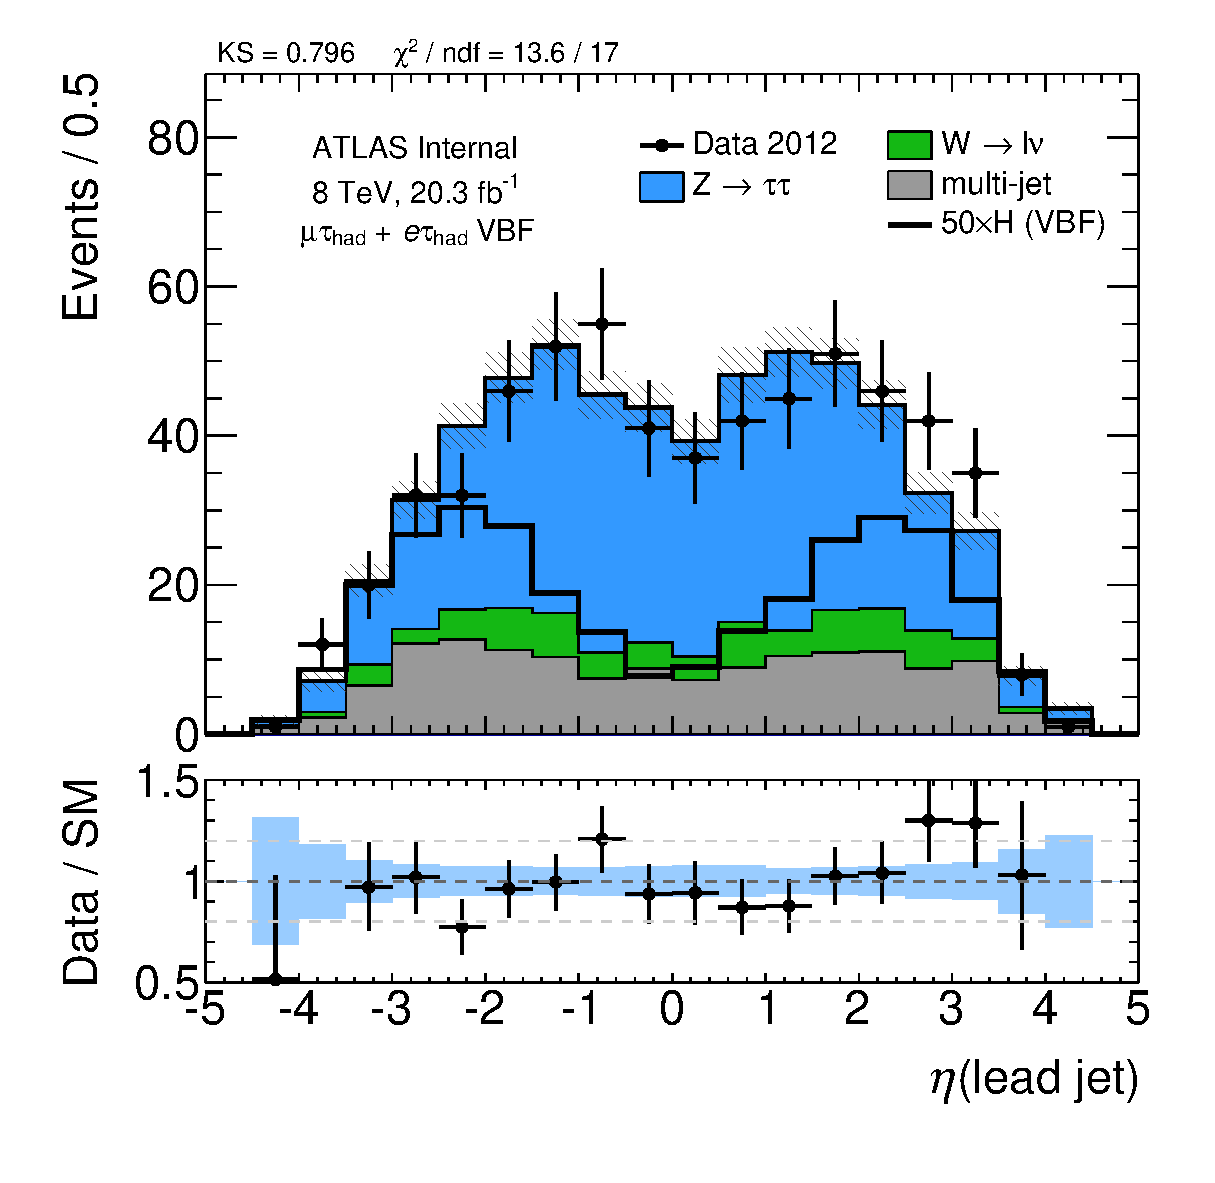
\includegraphics[width=0.32\textwidth]{figures/vbf-LTT/jet-1-eta}
  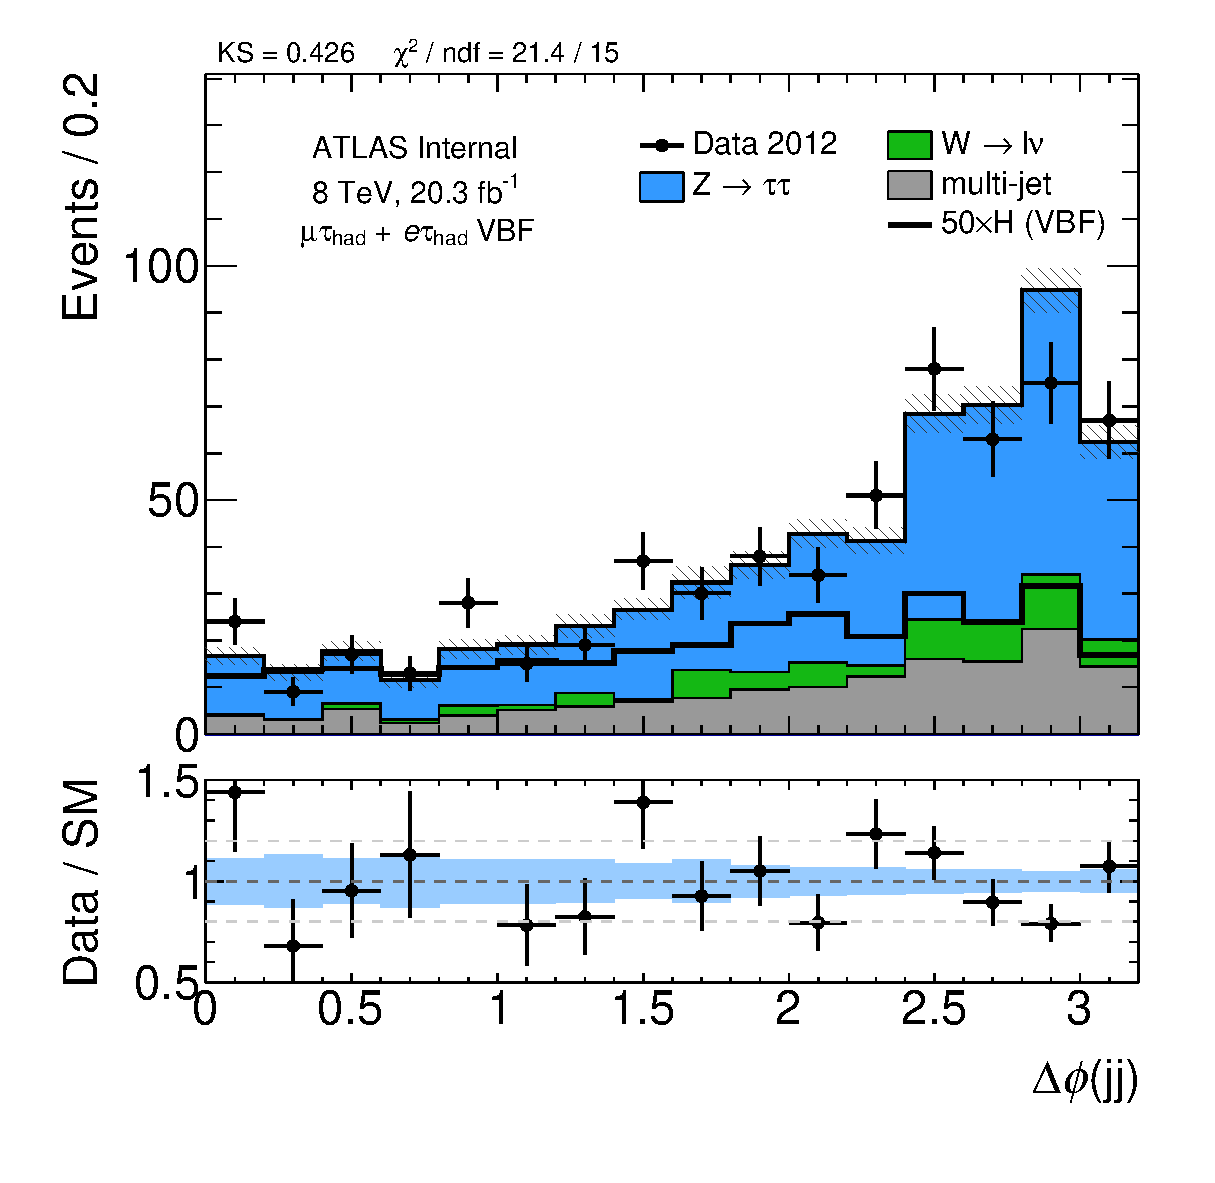
\includegraphics[width=0.32\textwidth]{figures/vbf-LTT/jets-dphi}
  % --------------
  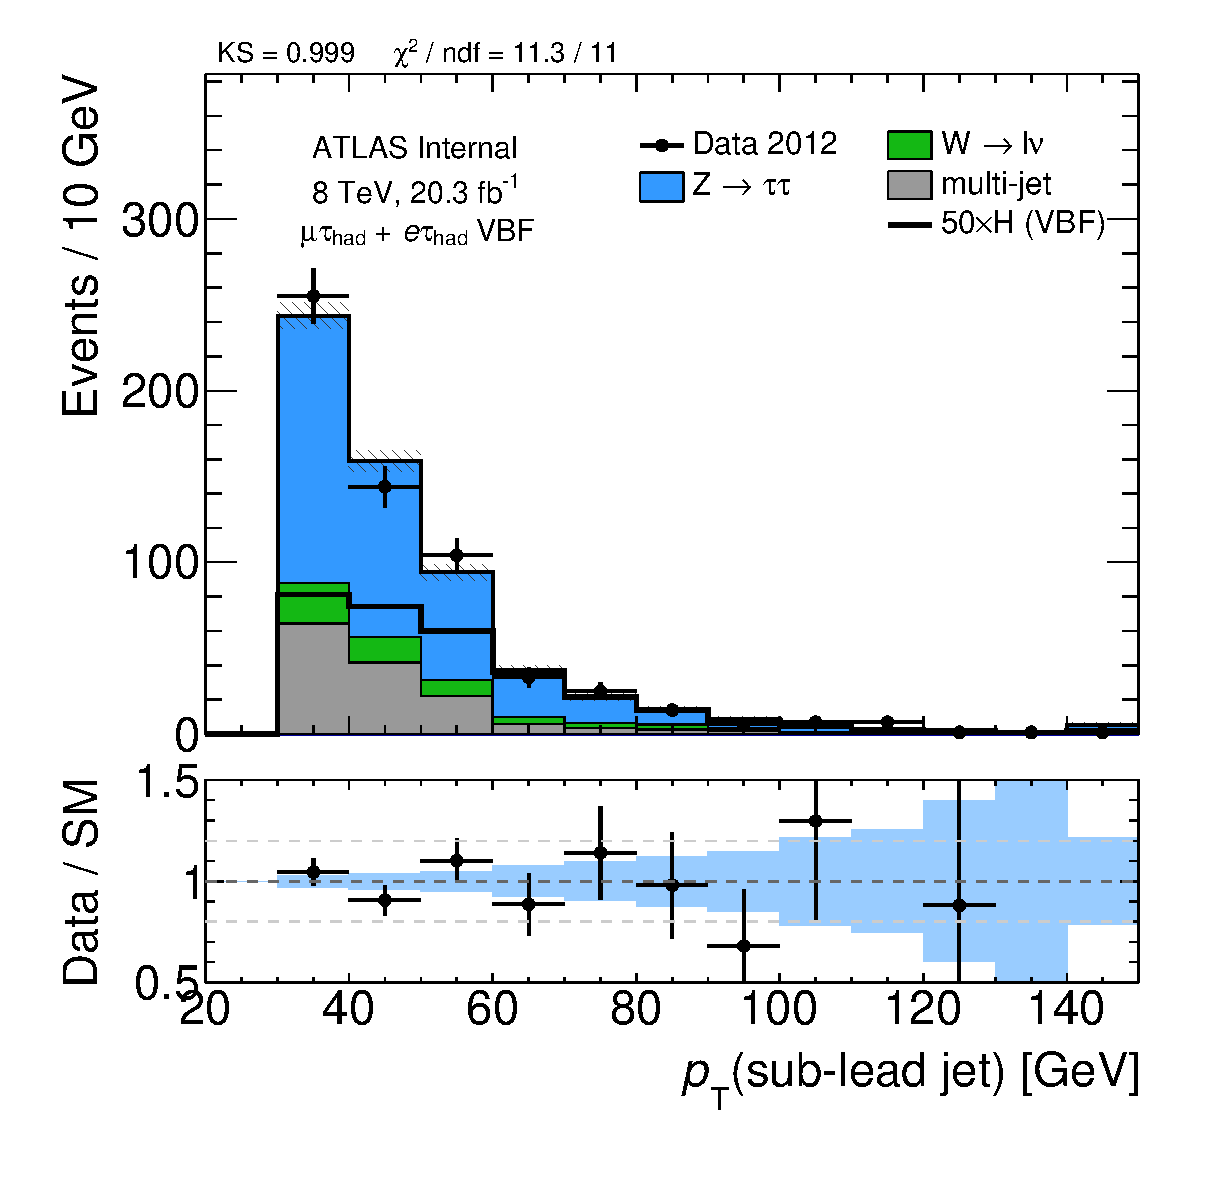
\includegraphics[width=0.32\textwidth]{figures/vbf-LTT/jet-2-pt}
  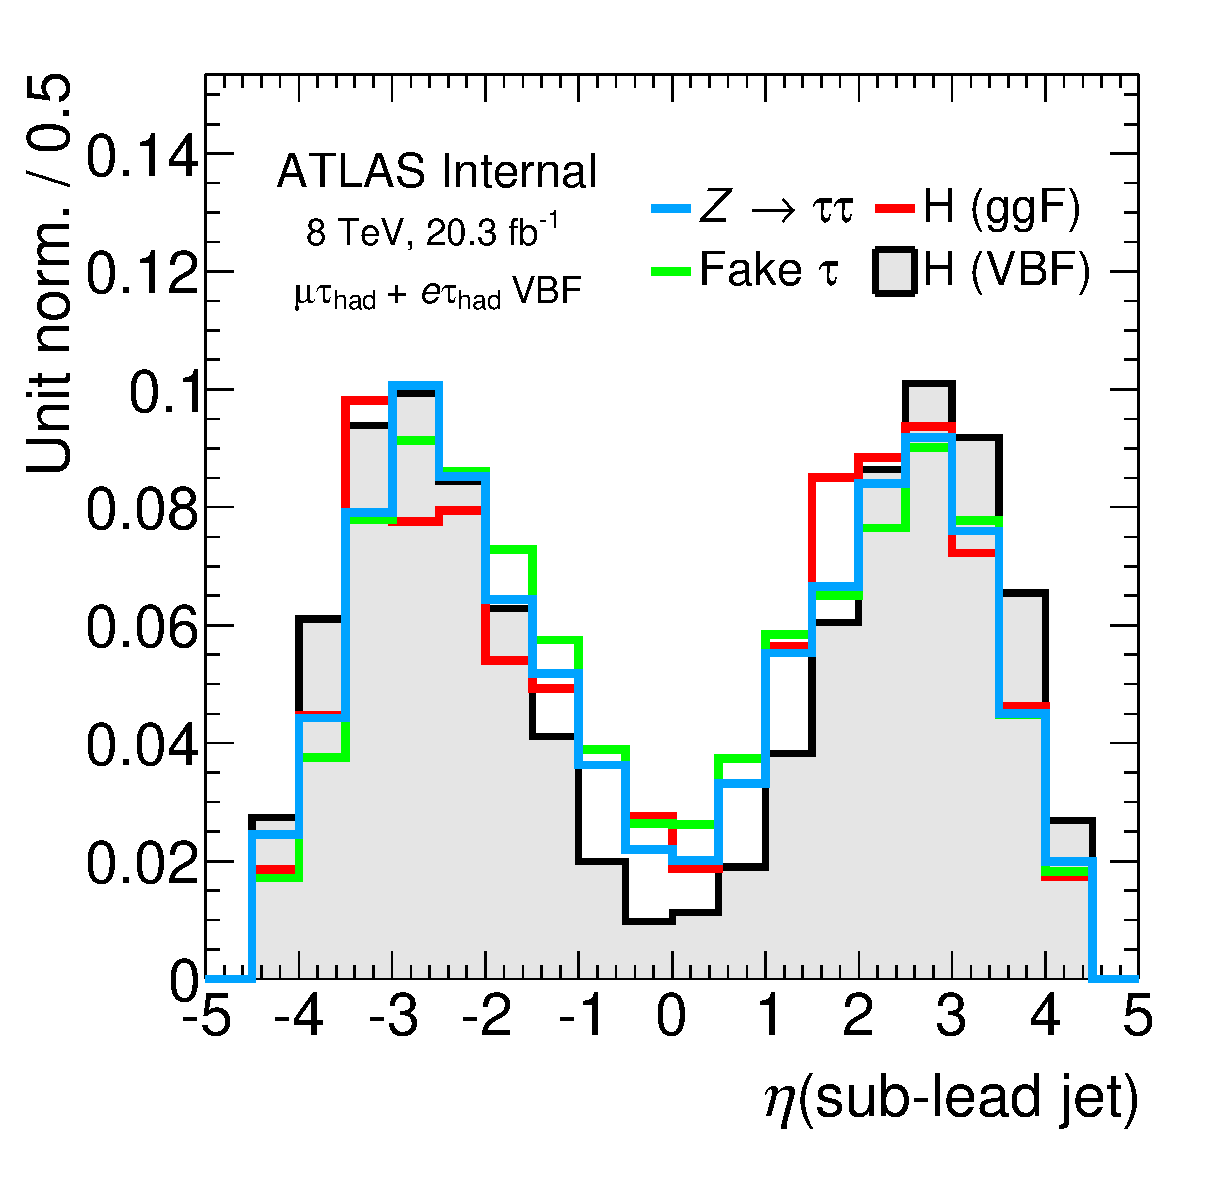
\includegraphics[width=0.32\textwidth]{figures/vbf-LTT/jet-2-eta}
  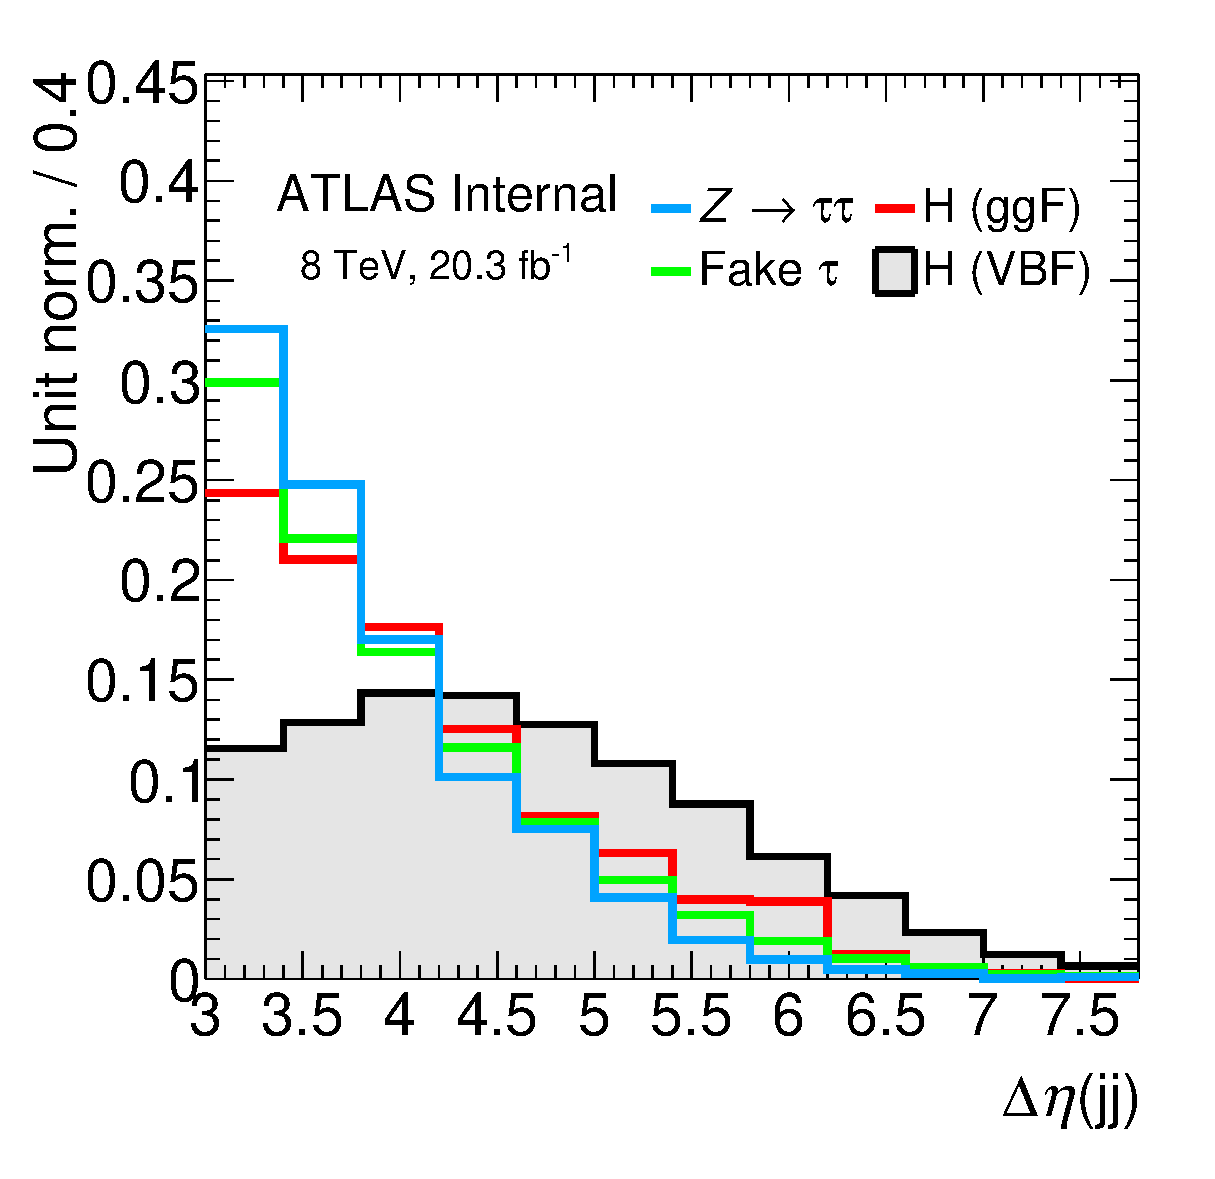
\includegraphics[width=0.32\textwidth]{figures/vbf-LTT/jets-deta}
  % --------------
  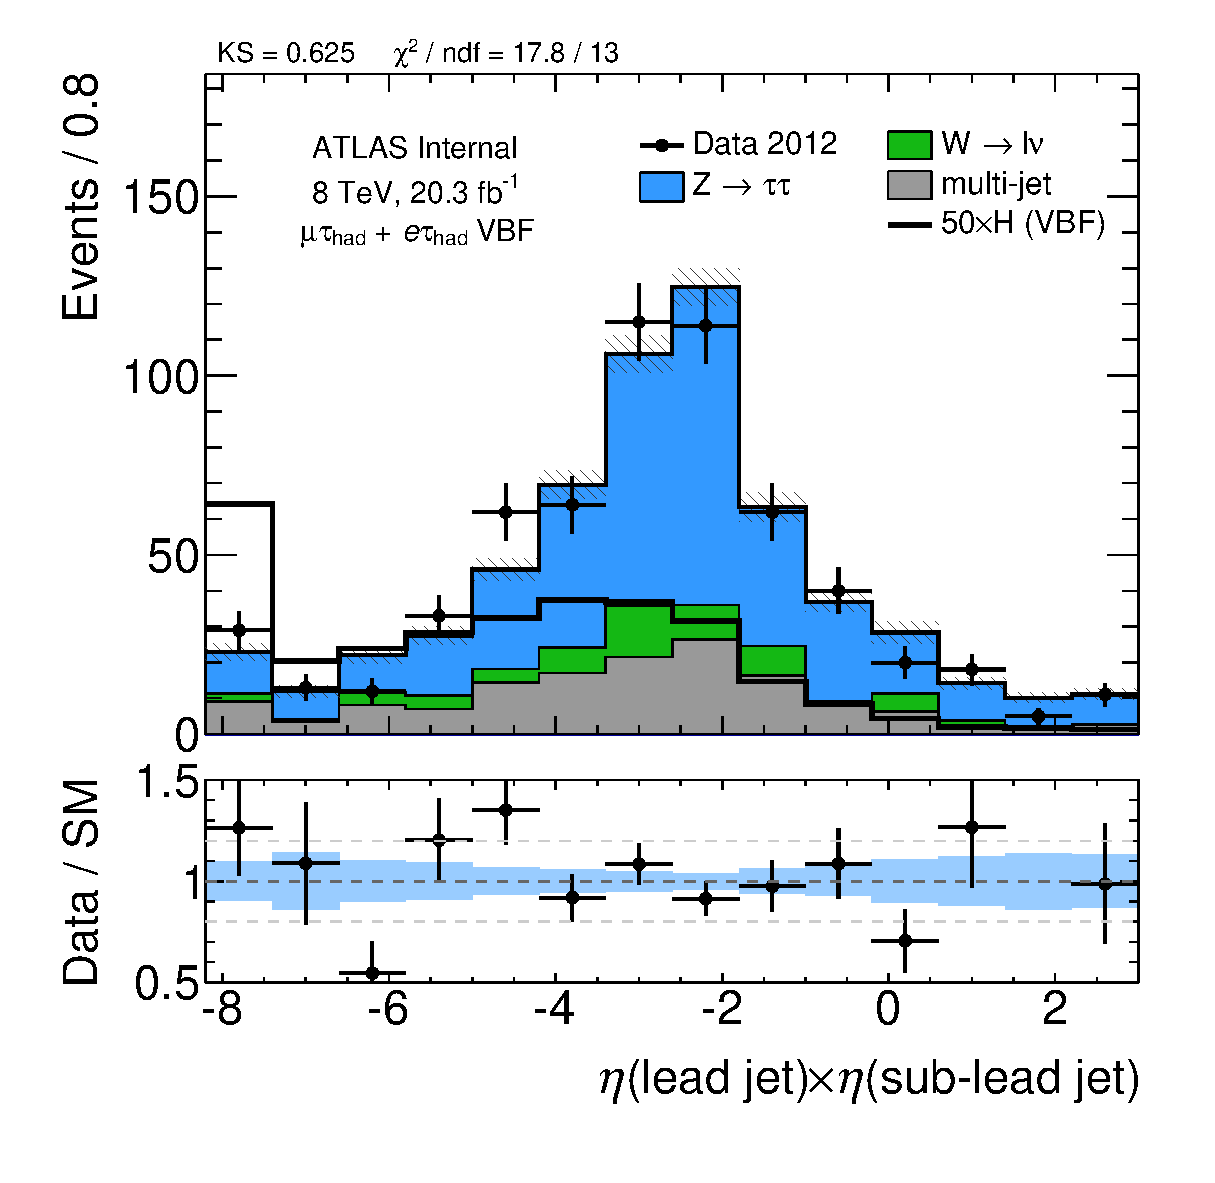
\includegraphics[width=0.32\textwidth]{figures/vbf-LTT/jets-etaprod}
  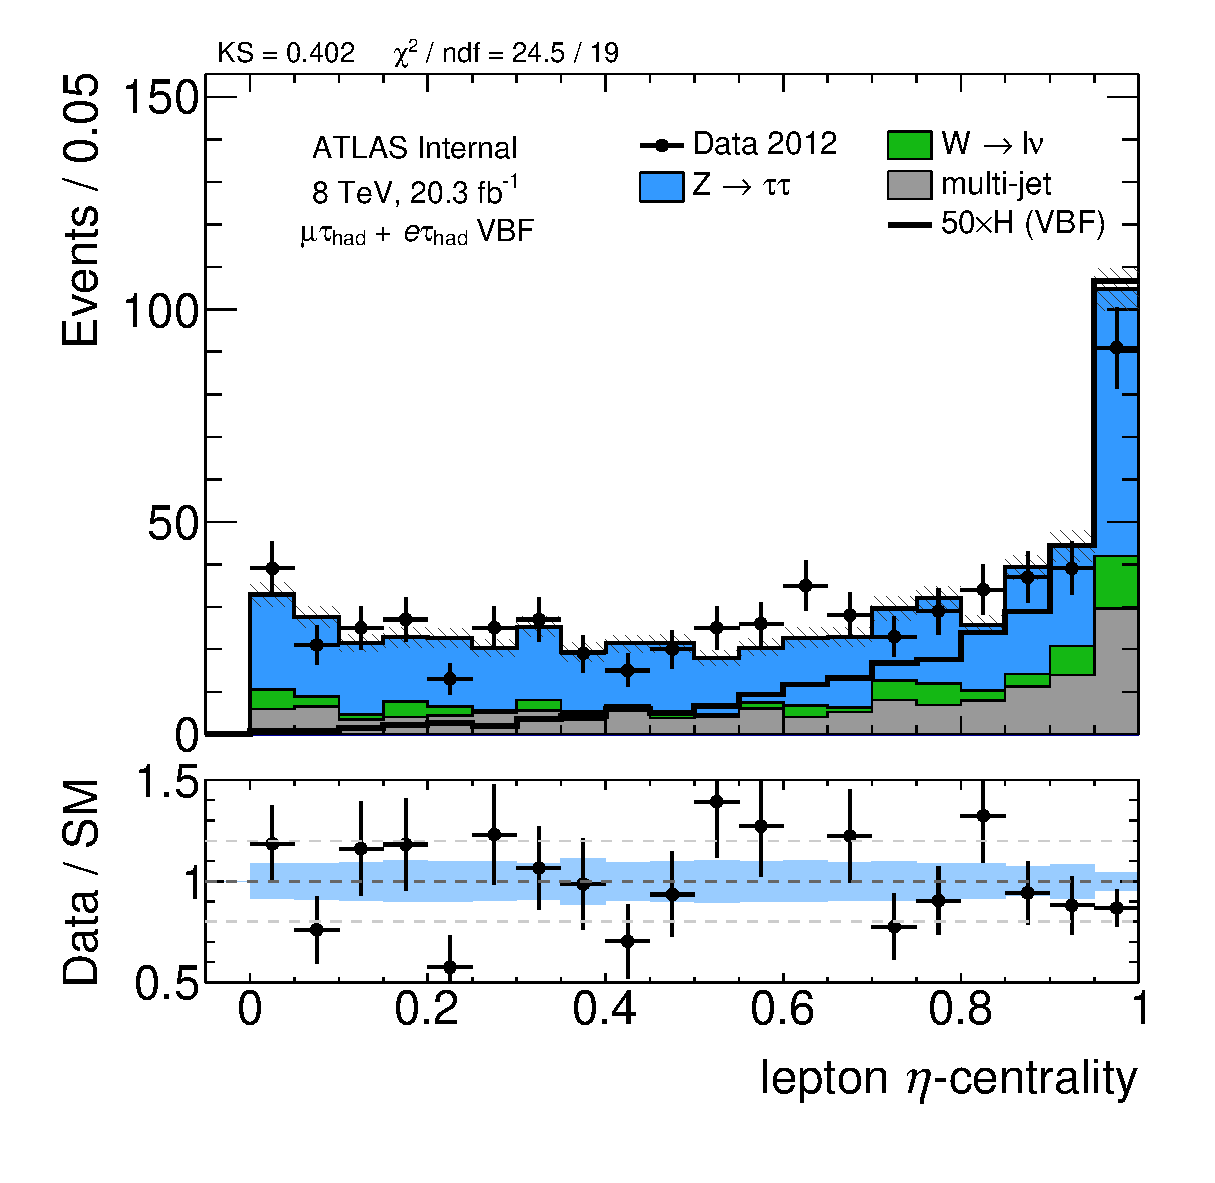
\includegraphics[width=0.32\textwidth]{figures/vbf-LTT/lep-eta-centrality}
  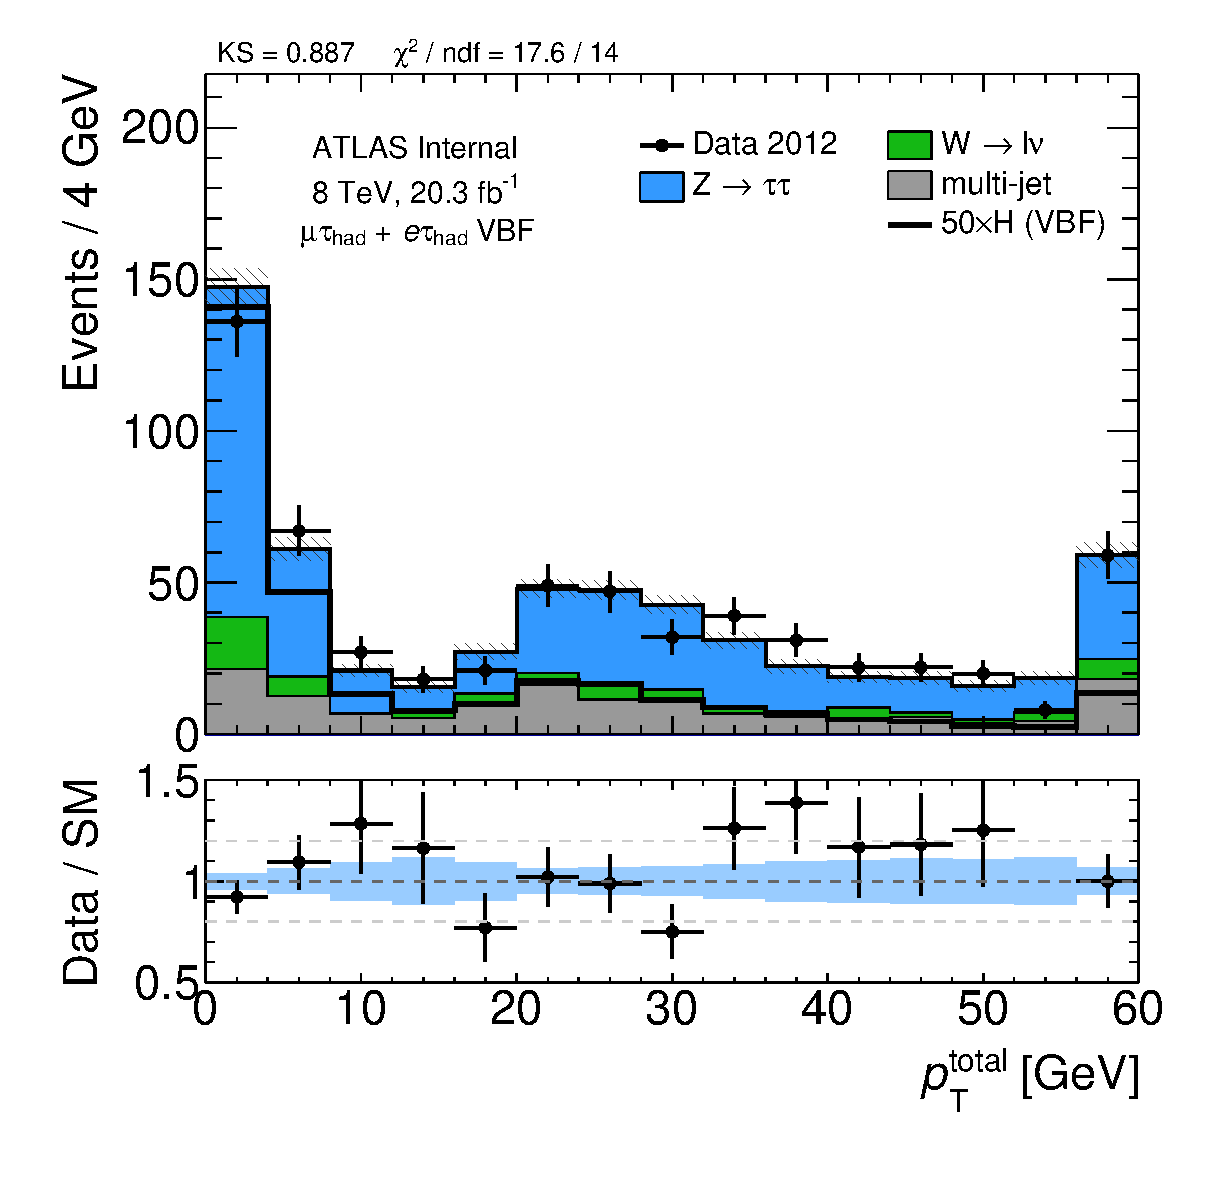
\includegraphics[width=0.32\textwidth]{figures/vbf-LTT/system-pt}
  % --------------
  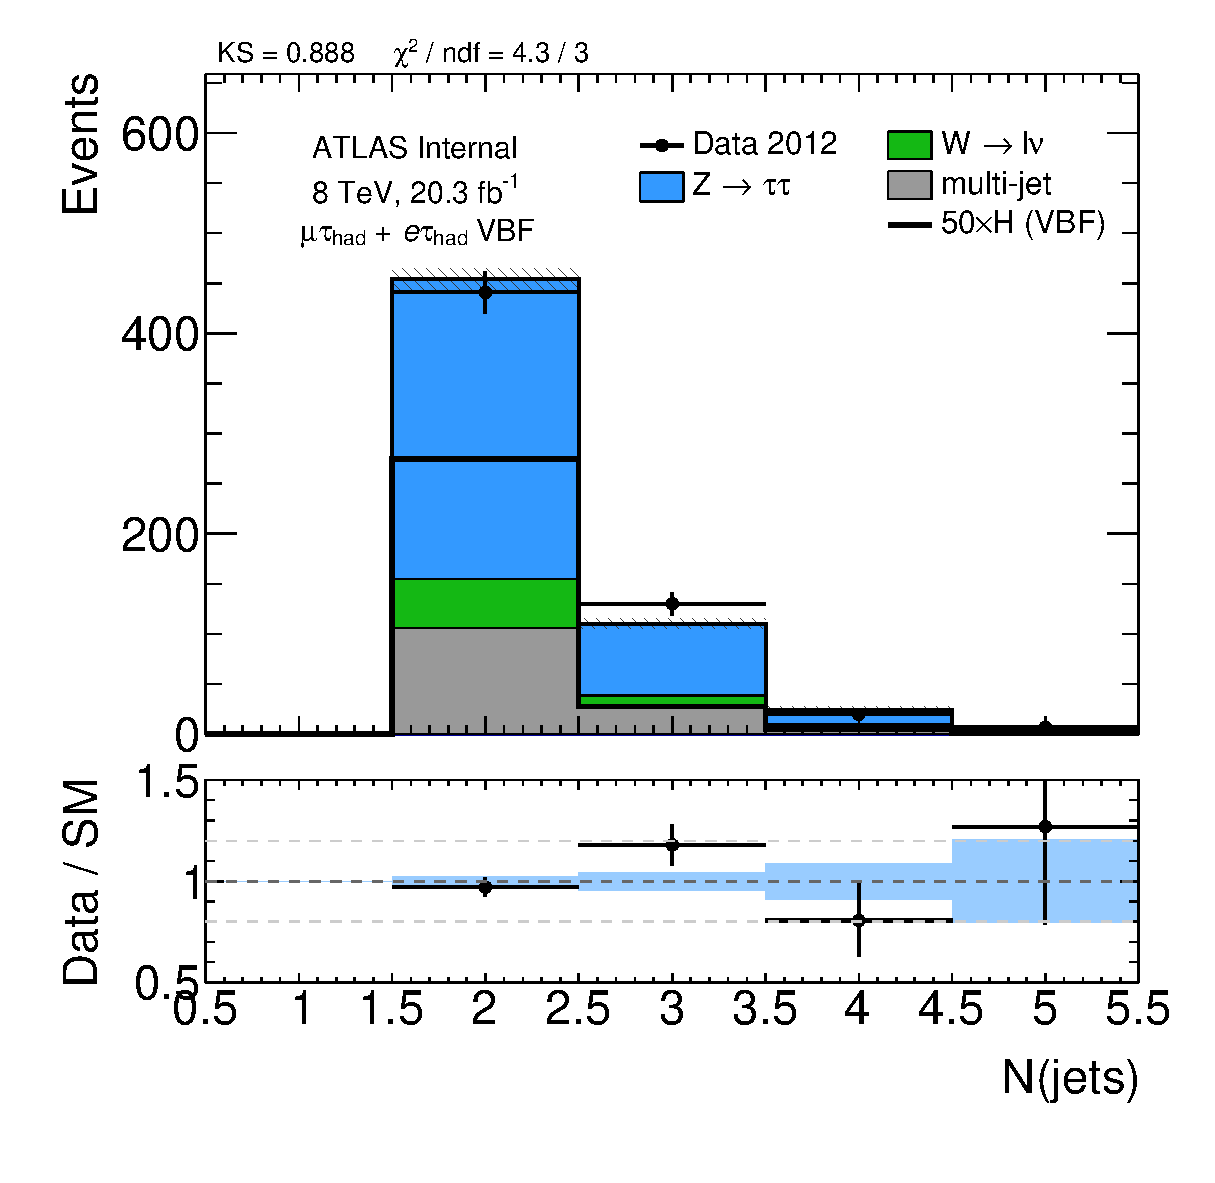
\includegraphics[width=0.32\textwidth]{figures/vbf-LTT/n-jets30}
  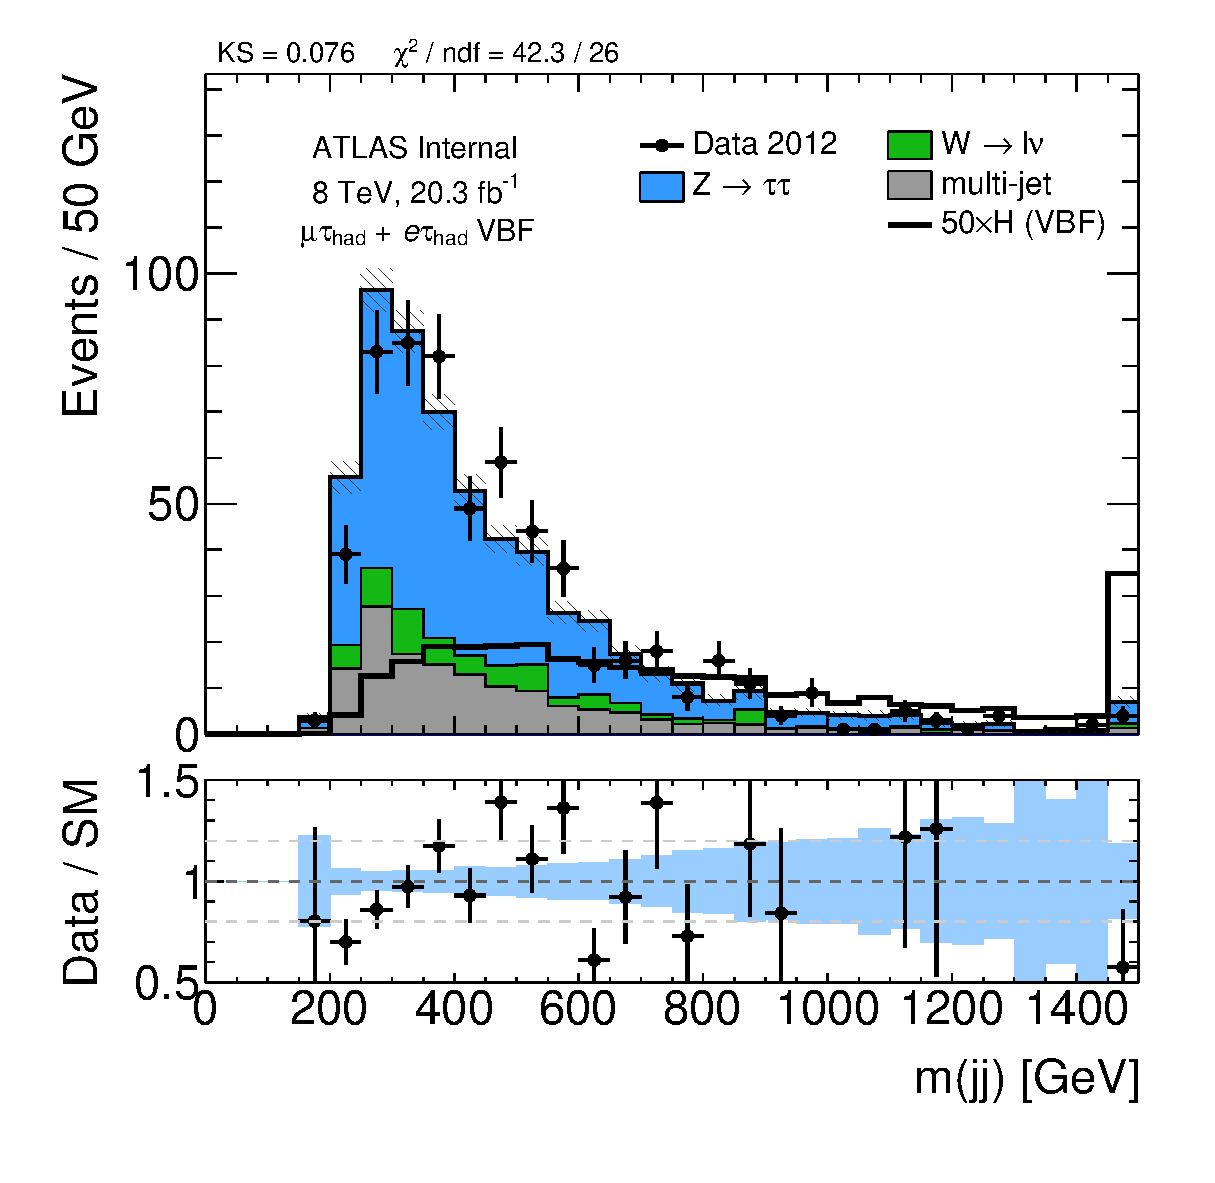
\includegraphics[width=0.32\textwidth]{figures/vbf-LTT/dijet-m-high}
  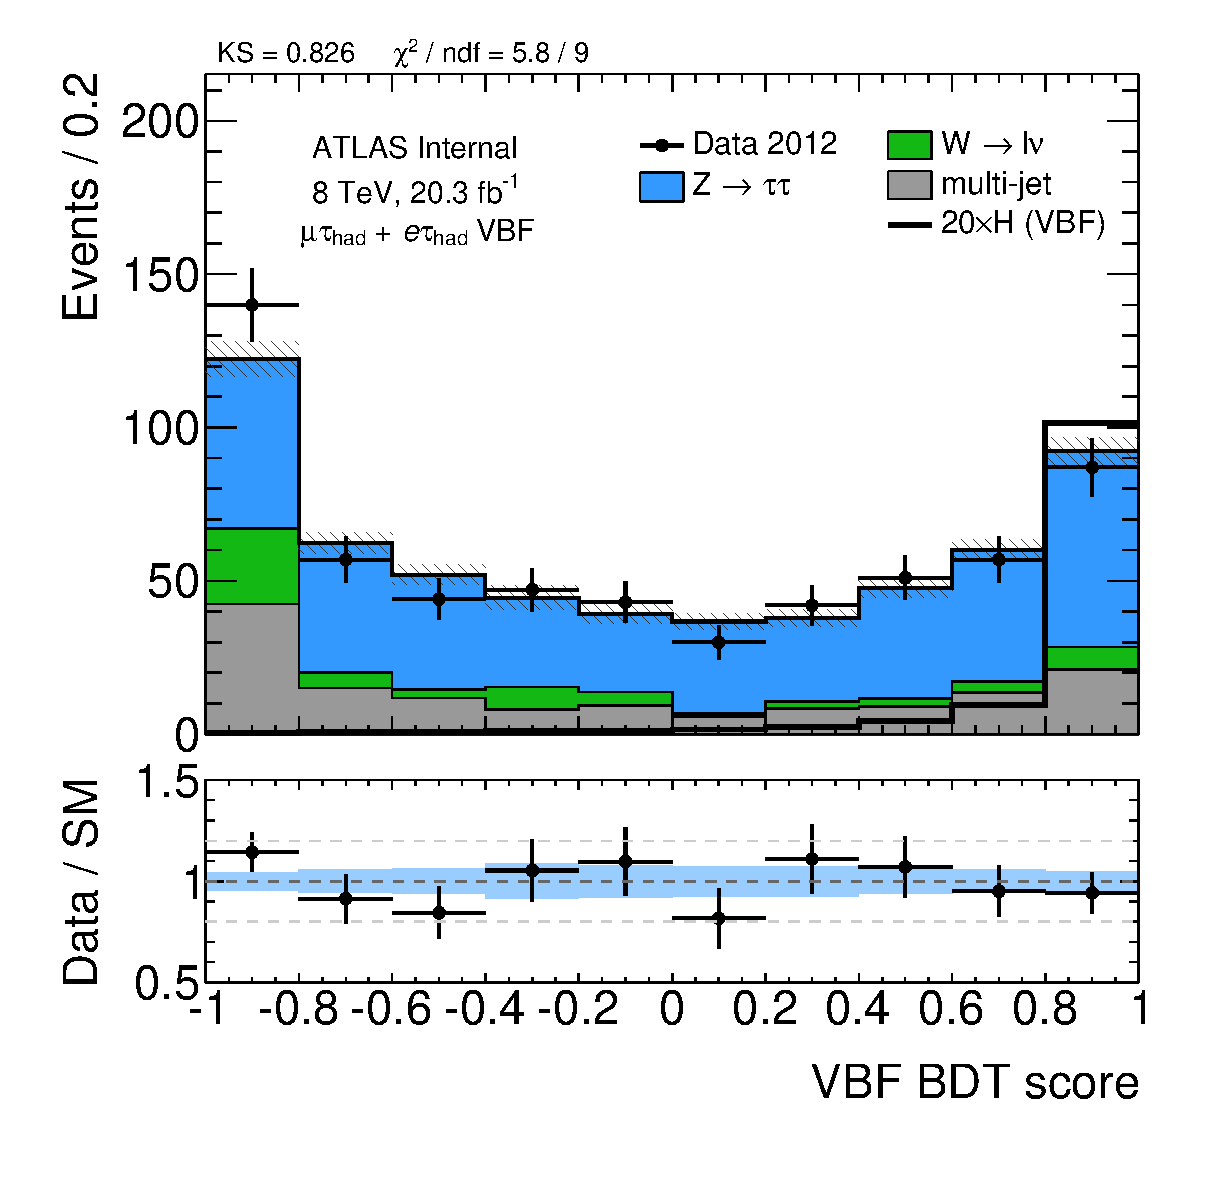
\includegraphics[width=0.32\textwidth]{figures/vbf-LTT/BDTEve-VBF}
  \caption{Variables.}
  \label{fig:prospects-ltt-jets}
\end{figure}
\clearpage

\subsection{Updates to the L1 $\tauh$ object}

Updates to the L1 $\tauh$ object are also considered. 

\subsubsection{Size}

The size of the L1 $\tauh$ is made larger to check if a sharper efficiency turn-on curve can be gained without significant background contamination. This is especially important for 3-track $\tauh$, which are expected to be wider than 1-track $\tauh$ and are observed to have a slower efficiency turn-on curve. The default L1 $\tauh$ used in 2012 data-taking is $2 \times 1$ in the electromagnetic calorimeter and $2 \times 2$ in the hadronic calorimeter.

Efficiency turn-on curves for various L1 $\tauh$ definitions are shown in \cref{fig:prospects-trigger-towersize} for simulated $\tauh$ with and without isolation requirements. A sharper efficiency turn-on is achieved relative to the default definition, but since background rates increase non-trivially, the default definition will be retained in 2015 data-taking.

\begin{figure}[!htpb]
  \centering
  \includegraphics[width=0.48\textwidth]{figures/trigger/turnon_L1TAU20_1p3p}
  \includegraphics[width=0.48\textwidth]{figures/trigger/turnon_L1TAU20I_1p3p}
  \caption{Variables.}
  \label{fig:prospects-trigger-towersize}
\end{figure}

\subsubsection{Isolation}

\begin{figure}[!htpb]
  \centering
  \includegraphics[width=0.48\textwidth]{figures/trigger/iso_background_noTAU60}
  \includegraphics[width=0.48\textwidth]{figures/trigger/iso_background_yesTAU60}
  \caption{Variables.}
  \label{fig:prospects-trigger-isolation-rate}
\end{figure}

\begin{figure}[!htpb]
  \centering
  \includegraphics[width=0.48\textwidth]{figures/trigger/iso_turnonL1_noTAU60}
  \includegraphics[width=0.48\textwidth]{figures/trigger/iso_turnonL1_yesTAU60}
  \caption{Variables.}
  \label{fig:prospects-trigger-isolation-turnon}
\end{figure}

\subsection{Conclusions and contingencies}



\clearpage
\section{HL-LHC}
\label{sec:prospects-hllhc}

\begin{figure}[tp]
  \centering
  \includegraphics[width=0.90\textwidth]{figures/PLOT-UPGRADE-2014-001/fig_08}
  \caption{Variables.}
  \label{fig:prospects-hllhc-layout}
\end{figure}

\begin{figure}[tp]
  \centering
  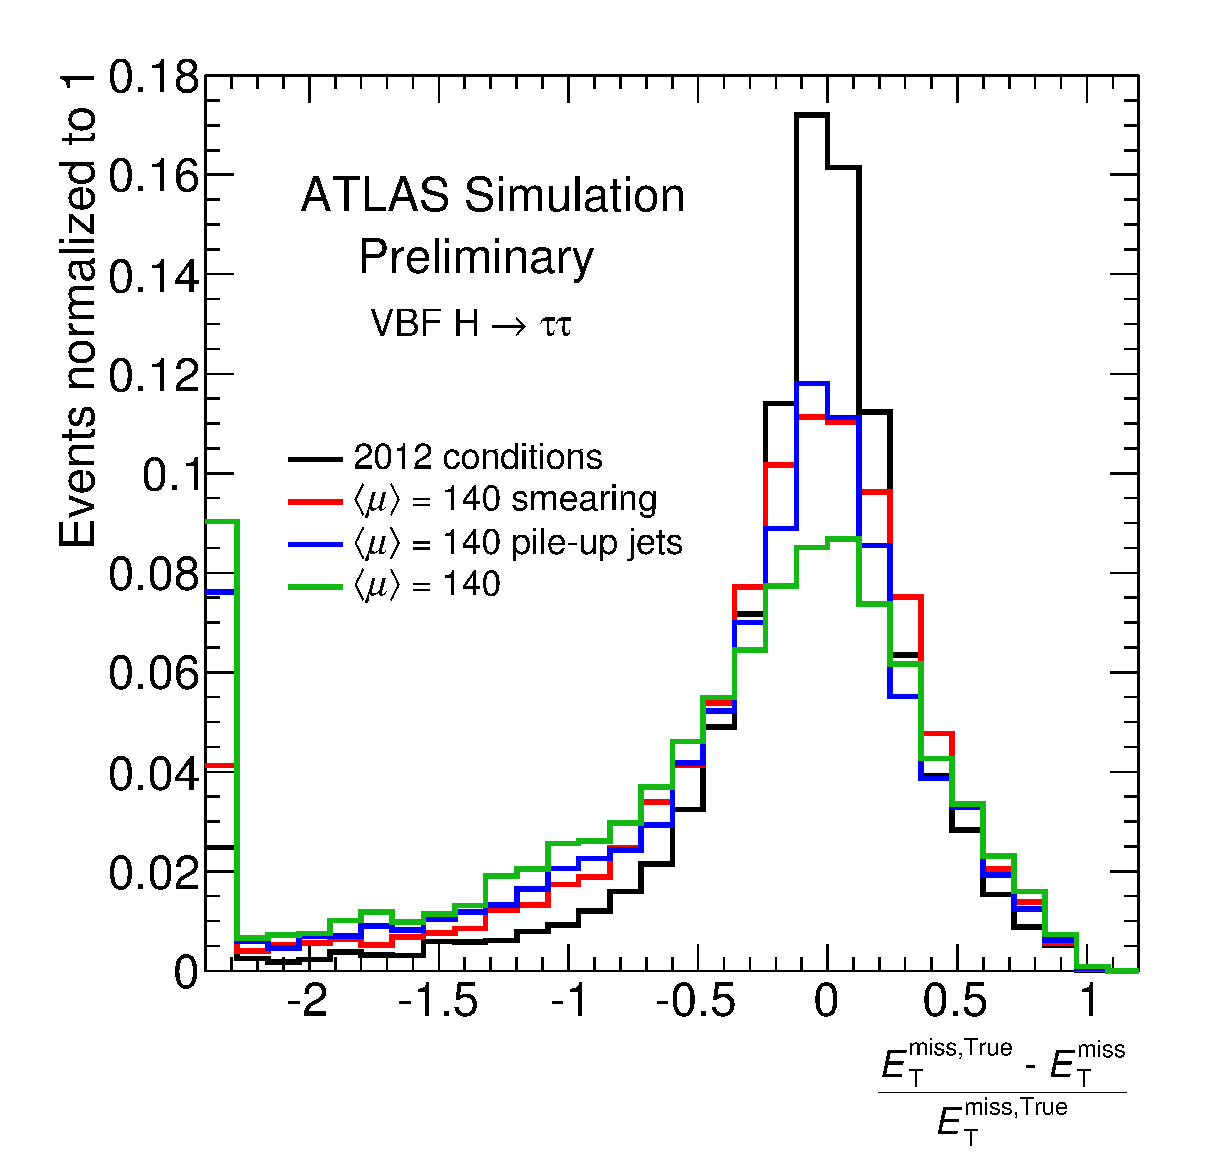
\includegraphics[width=0.48\textwidth]{figures/ATL-PHYS-PUB-2014-018/fig_01a}
  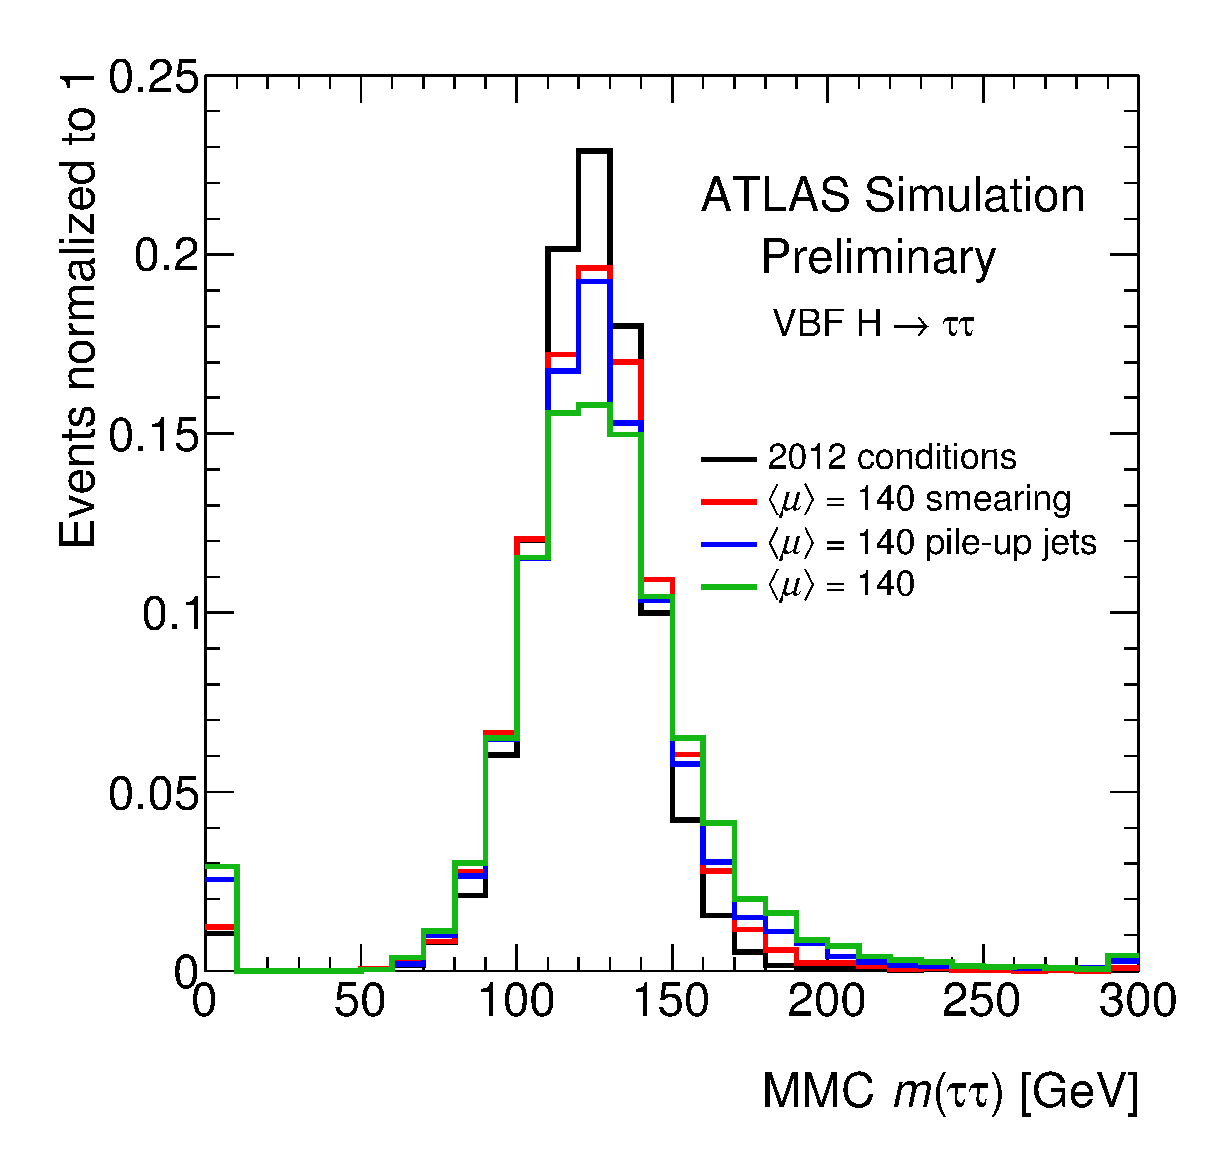
\includegraphics[width=0.48\textwidth]{figures/ATL-PHYS-PUB-2014-018/fig_01b}
  \caption{Variables.}
  \label{fig:prospects-hllhc-degradation}
\end{figure}

\begin{figure}[tp]
  \centering
  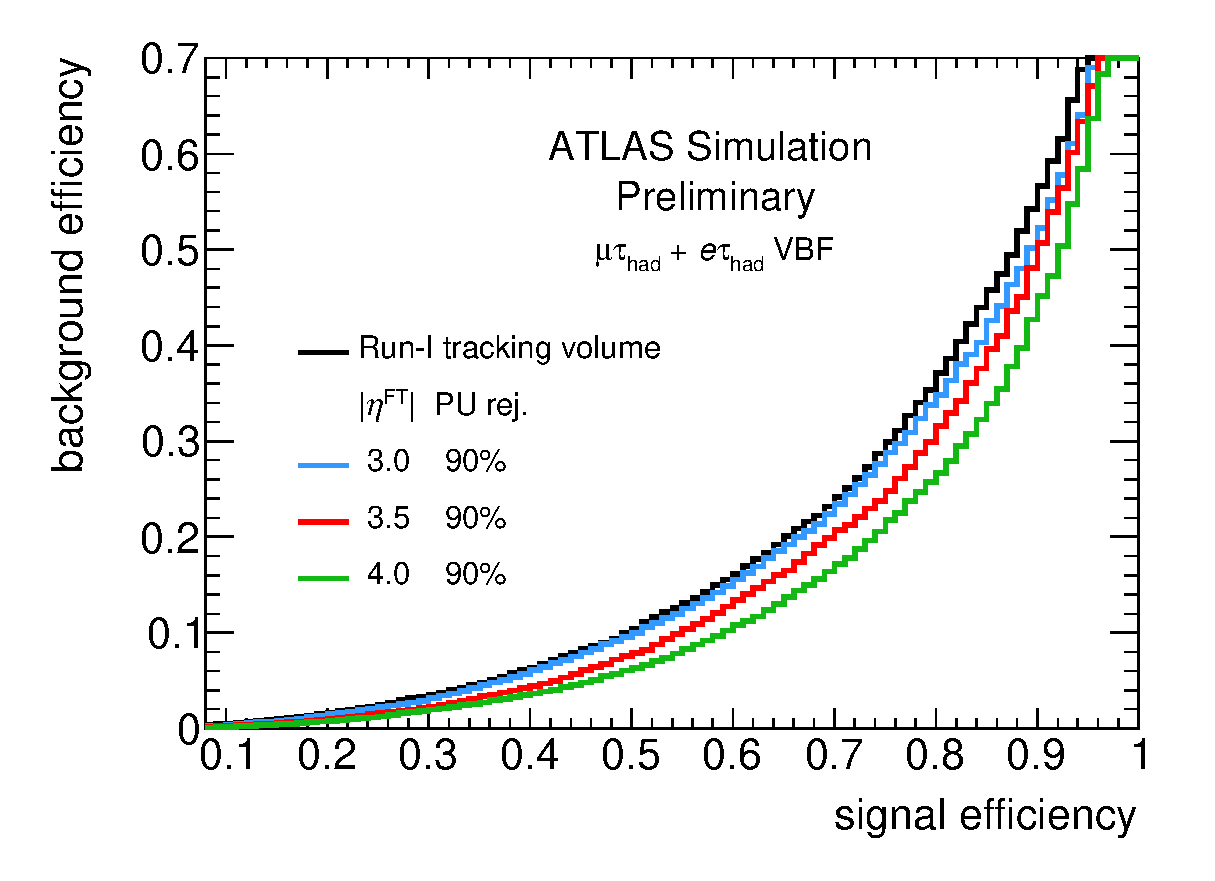
\includegraphics[width=0.48\textwidth]{figures/ATL-PHYS-PUB-2014-018/fig_02a}
  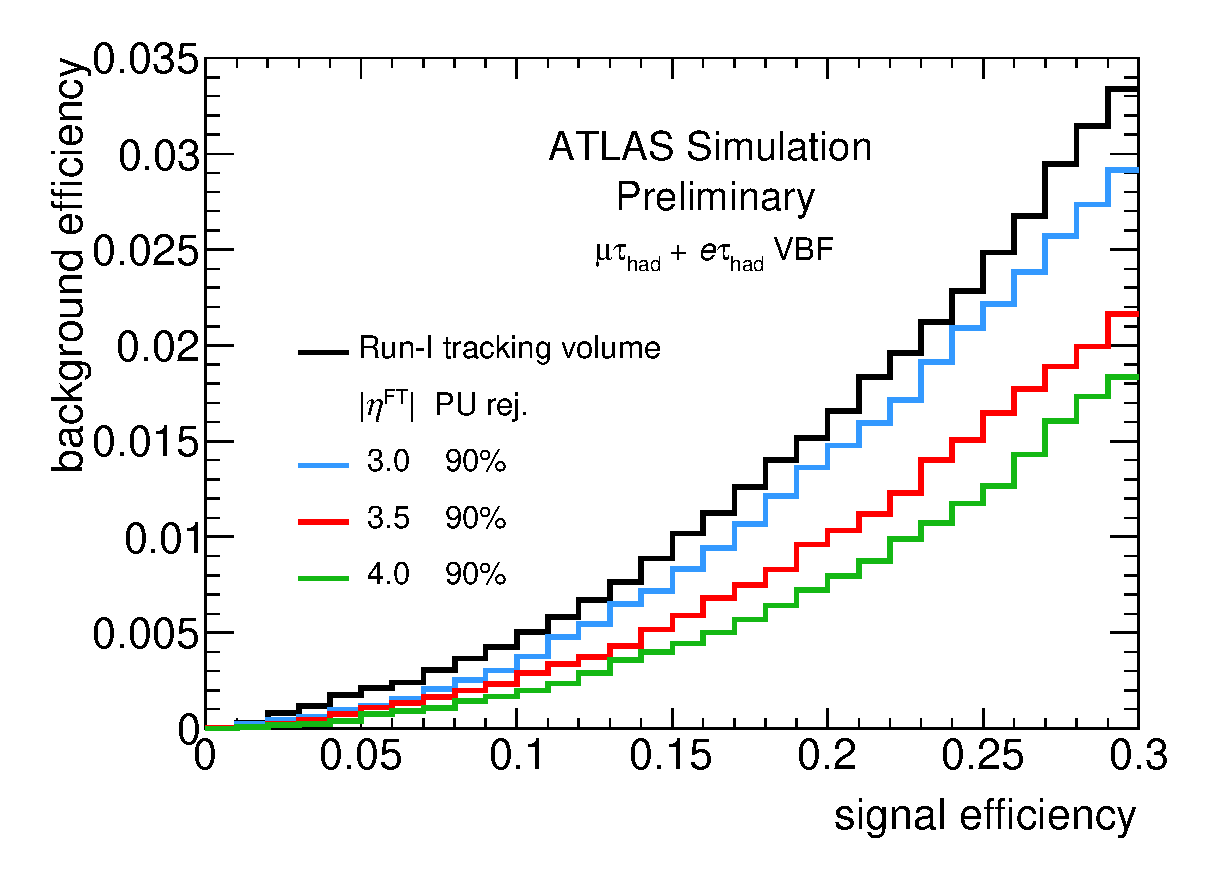
\includegraphics[width=0.48\textwidth]{figures/ATL-PHYS-PUB-2014-018/fig_02b}
  \caption{Variables.}
  \label{fig:prospects-hllhc-rocs}
\end{figure}

\begin{figure}[tp]
  \centering
  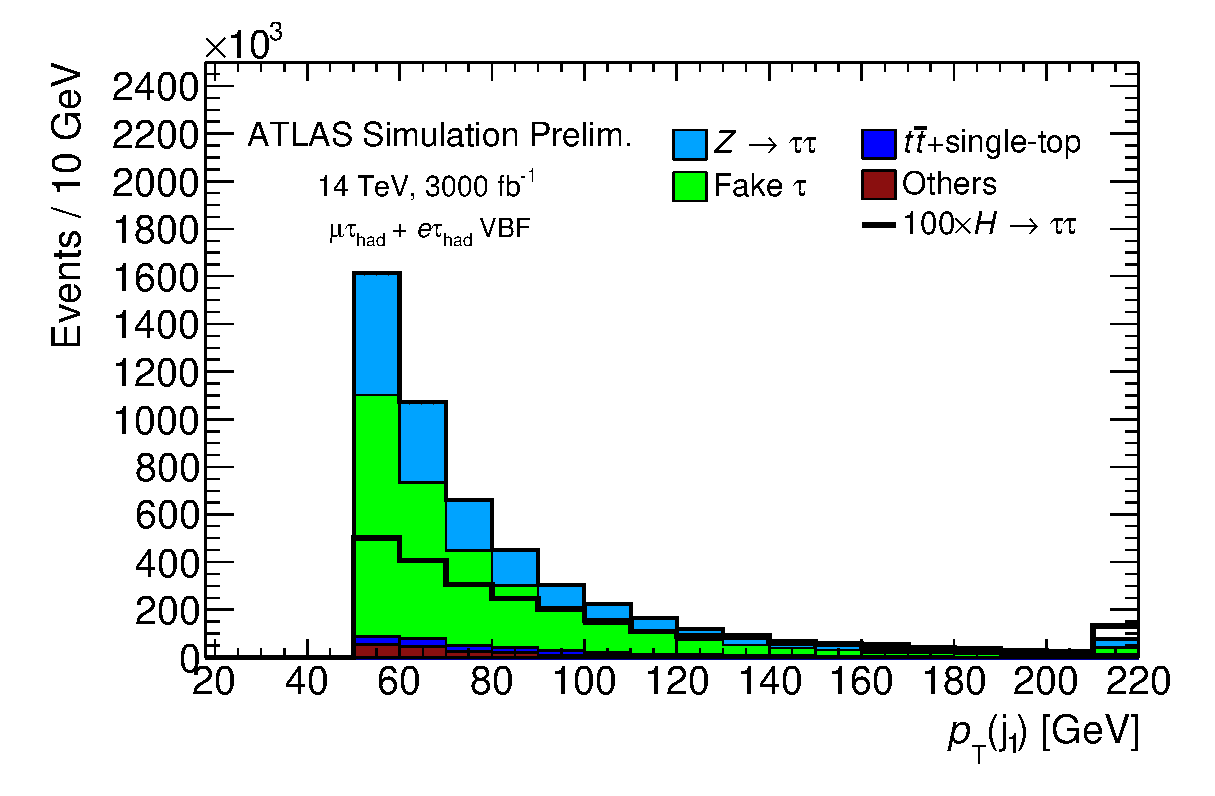
\includegraphics[width=0.48\textwidth]{figures/ATL-PHYS-PUB-2014-018/fig_03a}
  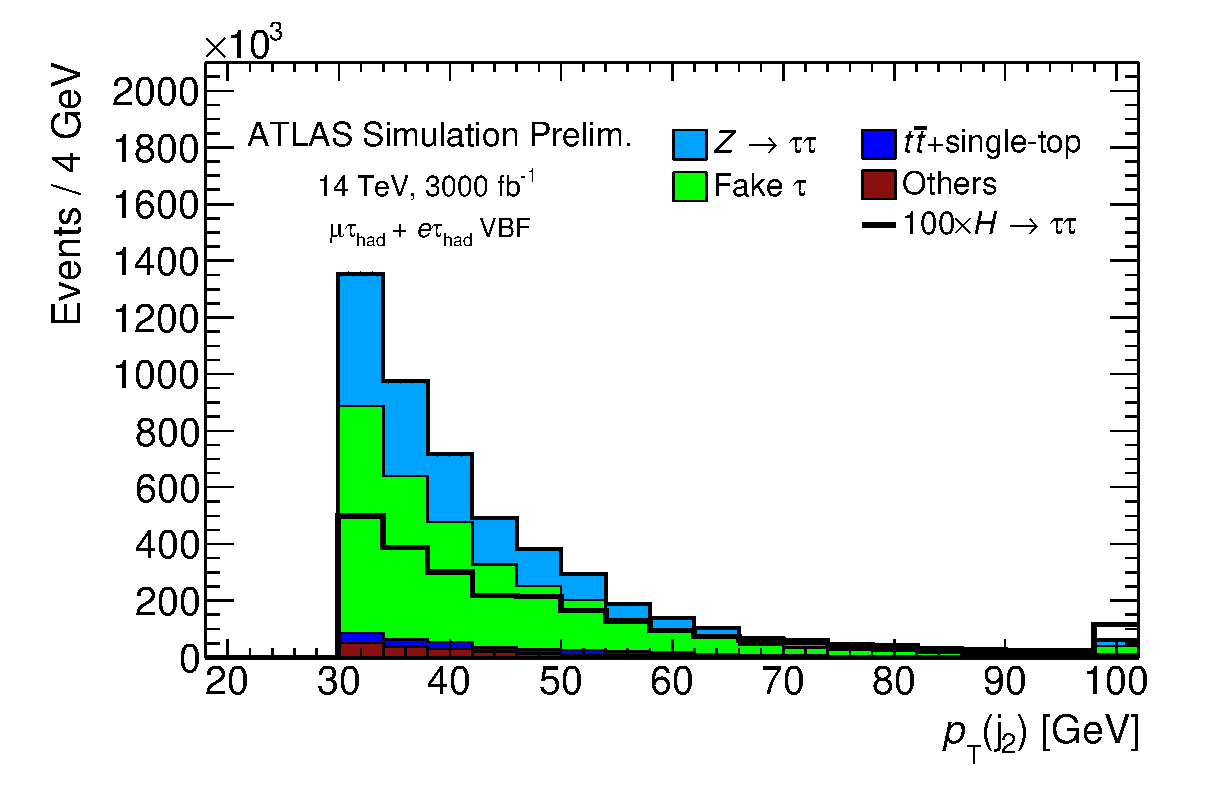
\includegraphics[width=0.48\textwidth]{figures/ATL-PHYS-PUB-2014-018/fig_03b}
  \includegraphics[width=0.48\textwidth]{figures/ATL-PHYS-PUB-2014-018/fig_03c}
  \includegraphics[width=0.48\textwidth]{figures/ATL-PHYS-PUB-2014-018/fig_03d}
  \includegraphics[width=0.48\textwidth]{figures/ATL-PHYS-PUB-2014-018/fig_03e}
  \includegraphics[width=0.48\textwidth]{figures/ATL-PHYS-PUB-2014-018/fig_03f}
  \includegraphics[width=0.48\textwidth]{figures/ATL-PHYS-PUB-2014-018/fig_03g}
  \includegraphics[width=0.48\textwidth]{figures/ATL-PHYS-PUB-2014-018/fig_03h}
  \caption{Variables.}
  \label{fig:prospects-hllhc-jets}
\end{figure}

\begin{figure}[tp]
  \centering
  \includegraphics[width=0.48\textwidth]{figures/ATL-PHYS-PUB-2014-018/fig_04a}
  \includegraphics[width=0.48\textwidth]{figures/ATL-PHYS-PUB-2014-018/fig_04b}
  \includegraphics[width=0.48\textwidth]{figures/ATL-PHYS-PUB-2014-018/fig_04c}
  \includegraphics[width=0.48\textwidth]{figures/ATL-PHYS-PUB-2014-018/fig_04d}
  \includegraphics[width=0.48\textwidth]{figures/ATL-PHYS-PUB-2014-018/fig_04e}
  \includegraphics[width=0.48\textwidth]{figures/ATL-PHYS-PUB-2014-018/fig_04f}
  \includegraphics[width=0.48\textwidth]{figures/ATL-PHYS-PUB-2014-018/fig_04g}
  \includegraphics[width=0.48\textwidth]{figures/ATL-PHYS-PUB-2014-018/fig_04h}
  \caption{Variables.}
  \label{fig:prospects-hllhc-taus}
\end{figure}

\begin{figure}[tp]
  \centering
  \includegraphics[width=0.48\textwidth]{figures/ATL-PHYS-PUB-2014-018/fig_06a}
  \includegraphics[width=0.48\textwidth]{figures/ATL-PHYS-PUB-2014-018/fig_06b}
  \caption{Variables.}
  \label{fig:prospects-hllhc-bdts}
\end{figure}


